\chapter{Entwurf} \label{chap:entwurf}

\section{Systemarchitektur} \label{sec:systemarchitektur}

In Abbildung \ref{fig:architecture} ist eine grobe Übersicht über die verschiedenen Komponenten des Projektes gegeben.
Es besteht aus drei Komponenten:
\begin{itemize}
	\item Hardware-Tracker
	\item Backend-Anwendung
	\item App
\end{itemize}

Der Hardware-Tracker ist die physische Komponente, die direkt an ein zu trackendes Papier angeheftet wird.
Er wird regelmäßig Daten erfassen und diese zur Lokalisierung an die Backend-Anwendung senden.

Die Backend-Anwendung dient als zentrales Element der Architektur.
Sie bekommt Daten des Trackers zugeschickt, wertet diese aus und speichert sie.
Auch das Management der Räume und Workflows wird von der Anwendung übernommen.

Nutzer verwenden zur Kommunikation mit dem Backend eine Smartphone-App.
Sie kommuniziert ebenfalls mit der Backend-Anwendung und fragt von dieser Informationen an oder löst Aktionen aus.

Die Entwürfe der drei Komponenten werden in den nachfolgenden Abschnitten im Detail erläutert.

Zusätzlich zu den drei Hauptkomponenten soll es eine Tool geben, dass das Setup eines Hardware-Trackers erleichtert.
Dieses Tool, genannt \enquote{Flasher}, dient zur Konfiguration der Firmware und dem Programmieren der Firmware auf die Hardware.

\begin{figure}[h!tbp]
	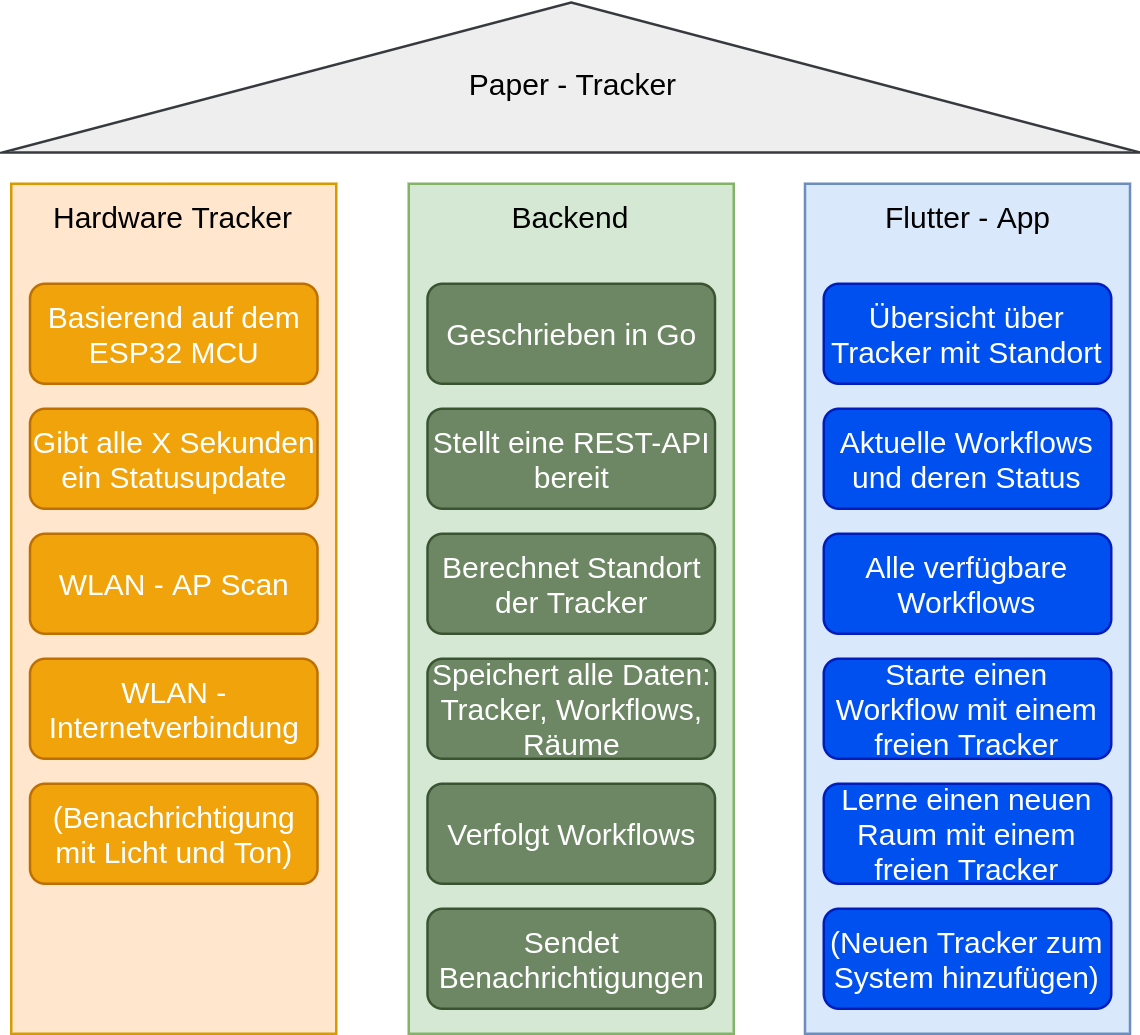
\includegraphics[width=\textwidth]{images/architecture_de.png}
	\centering
	\caption{Architektur des Paper-Tracker}
	\label{fig:architecture}
\end{figure}

\section{Komponentenarchitektur} \label{sec:komponentenarchitektur}

In den folgenden Abschnitten wird detaillierter auf die einzelnen Komponenten des in
\autoref{sec:systemarchitektur} beschriebenen Systems eingegangen.
Dabei werden die Komponenten in derselben Reihenfolge beschrieben, in welcher die Daten im
Gesamtsystem fließen.

\subsection{Tracking mit \glsentrylong{IoT}-Hardware} \label{sec:tracking-hardware}

Zur Erfassung der Standortdaten der Dokumente werden, wie in \autoref{sec:soll-analyse}
beschrieben, Hardware-Tracker eingesetzt.
Diese verwenden jedoch keine absolute Positionierungstechnologie wie beispielsweise \gls{GPS}, da
das hierfür benötigte Satellitensignal in Gebäuden zu schwach ist und somit die Positionierung
fehlschlagen kann.
\TODO{Quelle für die Genauigkeit von GPS in Gebäuden}

Für die Lokalisierung von Geräten innerhalb eines Gebäudes gibt es daher mehrere Ansätze, wie in
\autoref{sec:stand-der-forschung} beschrieben wurde.
Da die Positionsdaten ohnehin zur Auswertung an das Backend übertragen werden müssen, wofür eine
\gls{WLAN}-Verbindung notwendig ist, wird diese Methode eingesetzt.
Die gesammelten Daten werden dann im Anschluss an das Backend übermittelt.

Als Metrik für das Tracking über \gls{WLAN} können die in \autoref{sec:grundlagen-wlan} erläuterten
\gls{RSSI} oder \gls{RCPI} verwendet werden. Da diese Werte jedoch nicht unbedingt proportional zum
Abstand zum \gls{AP} wachsen oder fallen, da Funksignale durch unterschiedliche Materialien
unterscheidlich gedämpft werden, können sie nicht als absolut angesehen und verwendet werden.

Aus diesem Grund muss für jeden Raum die vorherrschende \gls{WLAN}-Umgebung in das System
\enquote{eingelernt} werden. Zu diesem Zweck gibt es einen eigenen Modus in der Anwendung, in
welchem ein ausgewählter Tracker ständig die verfügbaren \glspl{AP} und die zu diesen ermittelte
Signalstärke an den Server sendet. Dieser sammelt die Messwerte und aggregierte sie nach Abschluss
der Messung, also nach einem definierten Zeitintervall. Aggregriert werden die Metriken so, dass aus
den \gls{RSSI}-Werten für jeden \gls{AP} das Minimum und Maximum, sowie das erste und dritte Quartil
und Median und arithmetisches Mittel berechnet werden.

Soll nun ein Tracker lokalisiert werden, scannt dieser die aktuelle \gls{WLAN}-Umgebung und sendet
die Scanergebnisse an den Server. Dieser berechnet nun für jeden bereits eingelernten Raum einen
\textit{Score}. Der Score berechnet sich aus der Übereinstimmung der nun gemessenen \glspl{RSSI} mit
den vorher eingelernten. Hierfür wird über jeden für den Raum ermittelten \gls{AP} iteriert und
abhängig davon, in welches statistische Maß der neue Messwert fällt, Punkte vergeben. Die konkrete
Punkteverteilung ist hierbei noch nicht spezifiziert, es handelt sich um Parameter, welche genutzt
werden können, um die Genauigkeit des Trackings zu optimieren. Daher werden diese in
\autoref{chap:implementierung} beschrieben.

Die Kommunikation zwischen dem Tracker und dem Server läuft über Kommandos, die der Tracker sich beim Server abholt.
Dies ist in einem Sequenzdiagramm in \autoref{fig:tracker_comm} dargestellt.
Sobald der Tracker nach einem vorherigen Kommando aufwacht oder er zum ersten Mal gestartet wird, verbindet er sich zuerst
mit dem konfigurierten \gls{WLAN} Netzwerk.
Nachdem der Tracker verbunden ist, liest er seine zugewiesene Tracker ID aus dem Speicher.
Ist noch keine Tracker ID gespeichert, fordert er beim Server eine neue ID an.
Mit dieser ID kann der Tracker sich ein Kommando beim Server abholen.
Es gibt drei verschiedene Typen an Kommandos:
\begin{description}
	\item[SendTrackingInformation] \hfill \\
		Informationen über vorhandene \gls{WLAN}-Netzwerke an den Server schicken
	\item[SendInformation] \hfill \\
		Aktuellen Batteriestatus an den Server schicken
	\item[Sleep] \hfill \\
		Keine Aktion ausführen
\end{description}
Welcher Typ Kommando geschickt wird, entscheidet der Server je nach Status des Trackers.
Das Kommando wird direkt ausgeführt und dabei gegebenenfalls angefallene Ergebnisse an den Server geschickt.
Als Beispiel für ein Kommando ist das \enquote{SendTrackingInformation} weiter unten im Sequenzdiagramm dargestellt.

Mit dem Kommando erhält der Tracker zusätzlich eine Zeit, für die er schlafen soll.
Ist diese Zeit über einem bestimmten Grenzwert (z.B. 10 Sekunden) geht der Tracker in den sogenannten \enquote{Deep Sleep},
in welchem er möglichst wenig Strom verbraucht.
Wird dieser Grenzwert bei nur kurzen Zeiten nicht überschritten, wartet der Tracker die Zeit lediglich ab.
Dies verhindert ein ständiges Neuaufbauen der Verbindung zum \gls{WLAN}, welches sowohl Zeit als auch Strom kostet.
Nachdem entweder die Zeit im \enquote{Deep Sleep} oder wartend verbracht wurde, geht der Prozess wieder von vorne los.

\begin{figure}[]
	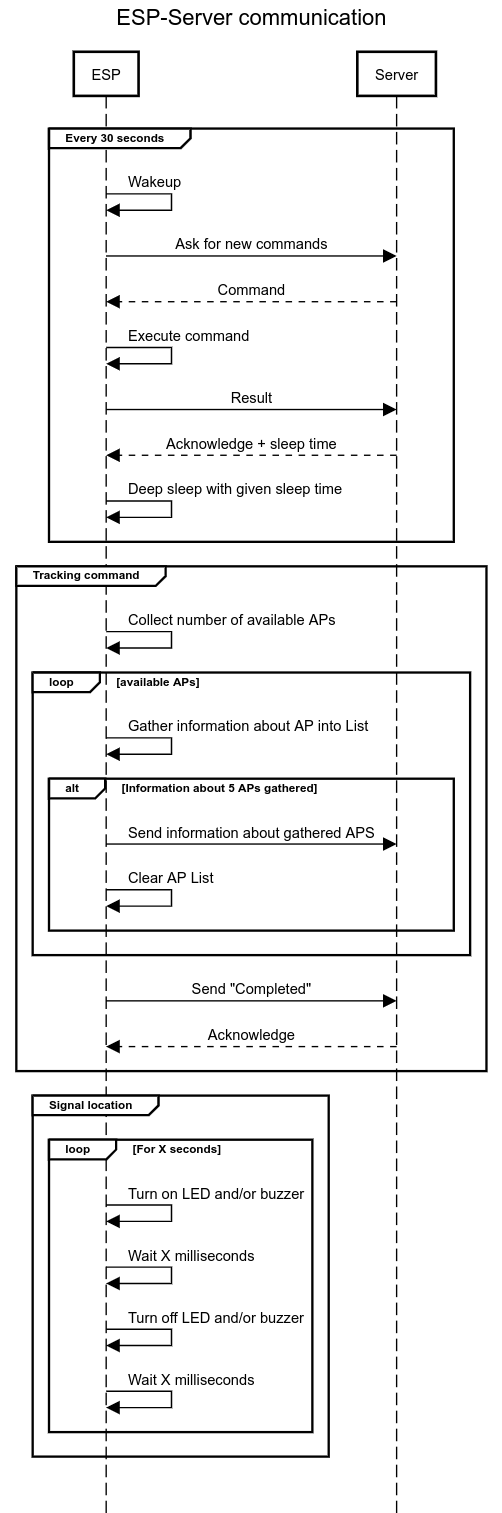
\includegraphics[height=0.9\textheight]{images/communication.png}
	\centering
	\caption{Sequenzdiagramm Kommunikation zwischen Tracker und Server}
	\label{fig:tracker_comm}
\end{figure}

\FloatBarrier
\subsection{Backend-Anwendung} \label{sec:backend}

\subsubsection{UML Daten Modellierung}
Da die Backend-Anwendung die zentrale Komponente des Systems ist und auch die Daten verwaltet, werden für sie die Daten-Klassen modelliert.
Das resultierende UML-Diagramm ist in Abbildung \ref{fig:uml} abgebildet.

Die zentrale Klasse des Diagramms bildet die \enquote{Tracker}-Klasse.
Sie modelliert einen Hardware-Tracker.
Einige Attribute des Trackers sind eine ID, das Label, der Batteriestatus, eine Flag, ob ein niedriger Batteriestatus notifiziert wurde
und einige Zeitstempel.
Die Zeitstempel geben zum Beispiel an, wann zuletzt ein Kommando abgeholt wurde oder wann zuletzt der Batteriestatus aktualisiert wurde.
Mit Hilfe der letzten dem Tracker gesendeten Zeit zum Schlafen kann mit der Funktion \enquote{GetSecondsToNextPoll()} abgefragt werden,
wann sich der Tracker vorraussichtlich das nächste Kommando abholt.
Neben den Attributen besitzt sie eine Referenz auf einen Status.
Dieser Status gibt an, zu was der Tracker zur Zeit verwendet wird und in welchen anderen Zustand gewechselt werden kann.

Es gibt vier verschiedene Zustände, die in Integern kodiert sind:
\begin{description}
	\item[Idle = 1] \hfill \\
		Tracker ist frei verfügbar und kann in \enquote{Learning} oder \enquote{Tracking} übergehen.
	\item[Learning = 2] \hfill \\
		Tracker wird für das Lernen eines Raumes verwendet und kann bei erfolgreichem Abschluss in \enquote{LearningFinished} oder bei Abbruch in \enquote{Idle} übergehen.
	\item[LearningFinished = 3] \hfill \\
		Das Lernen eines Raumes mit diesem Tracker wurde beendet. Die Ergebnisse können berechnet und einem Raum zugewiesen werden. In Folge darauf, geht der Tracker in den Zustand \enquote{Idle} über.
	\item[Tracking = 4] \hfill \\
		Der Tracker besitzt aktuell einen Workflow, den er trackt. Nach Abschluss dieses Workflows oder nach Abbruch, geht der Tracker in den Status \enquote{Idle} über.
\end{description}

Weiter besitzt der Tracker eine Referenz auf einen aktiven Workflow und den aktuellen Raum.
Beide Referenzen können nichtexistent sein, falls der Tracker keinen aktiven Workflow besitzt oder der Raum nicht bestimmbar ist.

Ein \enquote{Room} ist ein physikalischer Raum, der von einem Tracker erkannt werden soll.
Neben einem Identifizierer und einem \enquote{Label} (Name) für den Raum werden zusätzlich mehrere \enquote{BSSIDTrackingData} gespeichert.
Diese beinhalten für einen spezifischen \enquote{Access Point}/\gls{BSSID} einige Messdaten zu der gemessenen Signalstärke.
Über diese kann über eine Antwort des Trackers mit \enquote{ScanResults} die Position des Tracker bestimmt werden.

Damit der Tracker eine Antwort sendet, wird diese mit Hilfe eines Kommandos angefragt.
Diese Kommandos werden jeweils in einer Instanz der \enquote{Command}-Klasse abgebildet.
Die Kommandos besitzen einen spezifischen Typ der Enumeration \enquote{CommandType}, der die Aktion des Kommandos bestimmt.
Auch wird pro Kommando eine \enquote{SleepTimeSec} festgelegt, die bestimmt wie lange der Tracker sich nach der Aktion abschalten darf.

Spezielle Antworten der Tracker auf Kommandos und auch des Servers auf Anfragen der App sind in dem Unterpaket \enquote{communication} modelliert.
Dies ist zum Beispiel eine Fehler-Antwort und eine Basisklasse für Antworten des Trackers.
Diese \enquote{TrackerResponse}-Klasse besitzt auch ein Feld für den aktuellen Batteriestand des Trackers, um diesen überwachen zu können.

Unter den Klassen \enquote{WorkflowTemplate} und \enquote{WorkflowExec} sind die Workflows modelliert.
\enquote{WorkflowTemplate} stellt eine Blaupause dar, wie ein Workflow aussieht.
In diesem werden die einzelnen Schritte (\enquote{Steps}) des Workflows festgelegt.
Für einen \enquote{Step} werden ein Label und eine oder mehrere Referenzen auf dazugehörige Räume gespeichert.
Über die Klasse \enquote{NextStep} werden Referenzen auf nachfolgende Schritte modelliert.
Die \enquote{NextStep} Klasse besitzt ein Attribut \enquote{DecisionLabel}.
Ist diese ein leerer String, so ist dieser verbundene Schritt ein linearer.
Mit einem nicht-leeren String, gibt es mit diesem Schritt verschiedene Auswahlmöglichkeiten.
Durch das transitive Attribut \enquote{StepEditingLocked} der \enquote{WorkflowTemplate}-Klasse, wird die Bearbeitung blockiert.
Dieses Attribut ist gesetzt, sobald es eine Ausführung des Templates gab.

Die \enquote{WorkflowExec}-Klasse stellt einen konkreten Workflow in der Durchführung dar.
Als Attribute besitzt diese Klasse ein Label, einen Status und Start-/Endzeit.
Der Status ist entweder \enquote{Running}, \enquote{Completed} oder \enquote{Canceled}.
Weiter besitzt die Klasse eine Referenz auf das Template, das ausgeführt wird, eine Menge an \enquote{ExecStepInfo} und an den aktuellen Schritt.
Die Klasse \enquote{ExecStepInfo} besitzt Informationen über einzelne Schritte des Workflows.
Dies sind zum einen die Start-/Endzeit des Schrittes sowie, ob der Schritt übersprungen wurde, und zum anderen die \enquote{Decision}-Information.
Der \enquote{Decision} String wird im Falle von mehreren Auswahlmöglichkeiten in einem Workflow dazu genutzt, in der Ausführung den richtigen Weg zu wählen.

\begin{figure}[h!tbp]
	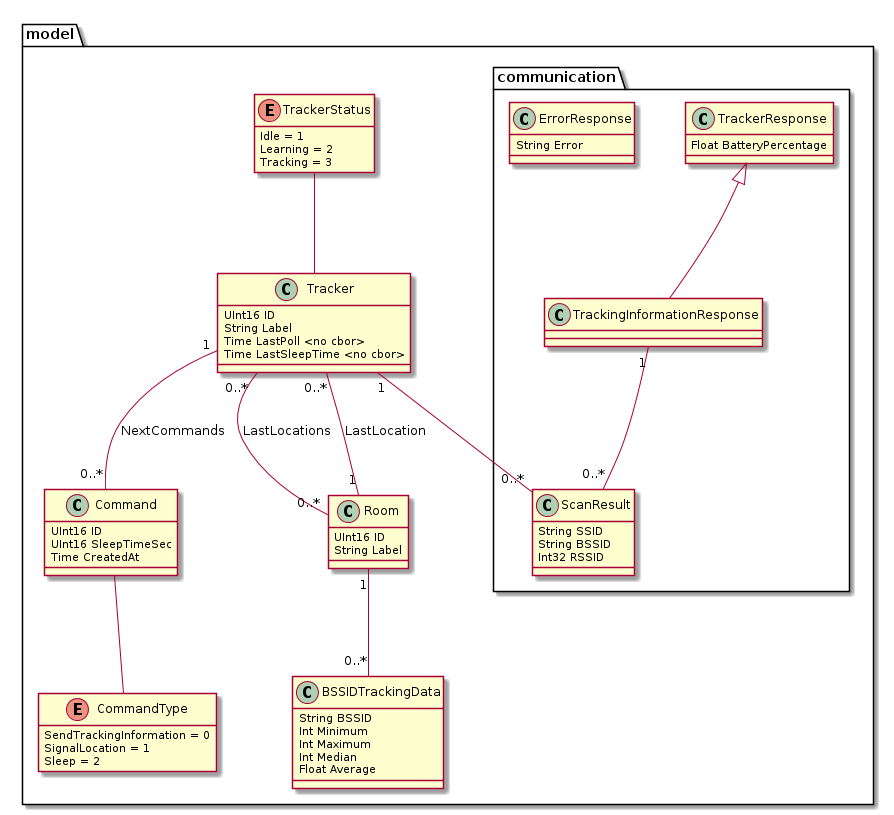
\includegraphics[width=\textwidth]{images/uml.png}
	\centering
	\caption{UML-Diagramm für die Backend-Anwendung}
	\label{fig:uml}
\end{figure}

\FloatBarrier

\subsubsection{Schnittstellen}

Für die Backend-Anwendung sind zwei verschiedene Schnittstellen vorgesehen.
Eine Schnittstelle ist für den Tracker und eine für die App vorgesehen.
Die unterschiedlichen Schnittstellen sollen die aus der Analyse entwickelten Ansprüche entsprechend erfüllen.

\paragraph{Tracker-Schnittstelle} \label{par:tracker-schnittstelle}
Für die Schnittstelle des Trackers bedeutet dies, dass sie möglichst simpel und effizient sein muss.
Dies wird über ein entsprechendes Protokoll und einem Datenformat erreicht.
Das verwendete Protokoll ist das \acrfull{CoAP} Protokoll und das Datenformat ist \acrfull{CBOR}.

Bei \gls{CoAP} handelt es sich um ein spezialisiertes Protokoll für die Verwendung in
\gls{IoT}-Hardware, welches dafür optimiert wurde möglichst wenig \gls{Overhead} zu haben.

Im \gls{IoT}-Bereich haben sich einige Protokolle durchsetzen können. Dazu zählen vor allem
\gls{HTTP}, \gls{MQTT}, \gls{AMQP} und \gls{CoAP}.
Da die Tracker batteriebetrieben sind, ist für diesen Anwendungsfall besonders die Performance des
eingesetzten Protokolles wichtig. Je weniger Overhead das Protokoll aufweist, desto weniger
Instruktionen müssen vom Prozessor des Trackers durchgeführt werden, was zu einer längeren Laufzeit
führt.
Werden die Protokolle anhand dieses Aspektes verglichen, erweist sich \gls{CoAP} als effizientestes
Protokoll. (vgl. \cite{Dizdarevic2019}, \cite{Naik2017})
\TODO{Quellen verwenden, die in diesem Paper zitiert werden}

\gls{CBOR} ist ein Datenformat, das auf kleine Code- und Nachrichtengrößen optimiert ist.
Demnach ist es auch für der \gls{IoT}-Bereich sehr gut geeignet.
Vom Aufbau des Formats, ist es sehr gut mit \gls{JSON} zu vergleichen, da es auch Schlüssel-Wert-Paare verwendet.
Der große Unterschied ist jedoch, dass \gls{CBOR} binär kodiert wird und \gls{JSON} in Text kodiert wird.
Dadurch ist \gls{CBOR} nicht menschenlesbar aber sehr gut maschinenlesbar.
Bei einem Vergleich zwischen der \gls{CBOR} Bibliothek \enquote{libCBOR} und der \gls{JSON} Bibliothek \enquote{ArduinoJson}
konnte zudem festgestellt werden, dass bei gleicher Nachricht das \gls{CBOR} Format ca. 26.5\% kleinere Nachrichten
in 83.3\% der Zeit schnellerer Zeit serialisiert hat.

Die Tracker-Schnittstelle soll drei Endpunkte zur Verfügung stellen.
Diese sind in \autoref{tab:coap-api} aufgelistet.
Bis auf den Endpunkt zum Erstellen eines neuen Trackers, erhalten alle Endpunkte als Parameter die Tracker ID des Trackers, der die Anfrage stellt.
Der Endpunkt zum Speichern der Trackingergebnisse hat zudem als Parameter die Ergebnisse selbst.

\begin{table}[]
\begin{tabular}{l l l l}
\textbf{Verb} & \textbf{Pfad}     & \textbf{Aktion}                   & \textbf{Rückgabewert}    \\ \hline
POST          & /tracker/new      & Neuen Tracker erstellen           & Tracker ID \\ \hline
GET           & /tracker/poll     & Kommando für Tracker abfragen     & Tracker Kommando   \\ \hline
POST          & /tracker/tracking & Ergebnisse des Tracking speichern & -
\end{tabular}
\caption{\label{tab:coap-api}Verfügbare Endpunkte der Tracker-Schnittstelle}
\end{table}

\FloatBarrier
\paragraph{App-Schnittstelle} \label{par:app-schnittstelle}
Die Schnittstelle für die App hat keine besonderen Anforderungen und kann daher frei gewählt werden.
Aus diesem Grund werden Protokolle und Datenformate verwendet, die momentan dem aktuellen Stand der
Technik entsprechen. \TODO{Quelle für aktuelle Protokolle}
Daraus ergibt sich der Vorteil, dass sie mit allen anderen gewählten Technologien sehr gut
kombinierbar sind und entsprechende Bibliotheken vorhanden sind.
Das verwendete Protokoll ist das \gls{HTTP}-Protokoll und das Datenformat ist \gls{JSON}.
Die Schnittstelle basiert auf dem \gls{REST} Paradigma (vgl. \cite{Fielding2000}). \TODO{Soll REST erläutert werden?}
Alle verfügbaren Endpunkte der App-Schnittstelle sind in \autoref{tab:http-api} dargestellt.

\begin{footnotesize}
\begin{landscape}
	\begin{longtable}{l|l|l|l|l}
		\caption{Liste aller Endpunkte der App-Schnittstelle \label{tab:http-api}} \\
\textbf{Verb} & \textbf{Pfad} & \textbf{Aktion} & \textbf{Parameter} & \textbf{Rückgabewert} \endfirsthead \hline
\textbf{Verb} & \textbf{Pfad} & \textbf{Aktion} & \textbf{Parameter} & \textbf{Rückgabewert} \endhead \hline
\multicolumn{5}{c}{\textit{Räume}} \\ \hline
\texttt{GET}    & \texttt{/room}     & Auflistung der Räume        & -    & Liste aller Räume                                                       \\ \hline
\texttt{POST}   & \texttt{/room}     & Erstellen eines neuen Raums & Raum & Erstellter Raum                                                         \\ \hline
\texttt{PUT}    & \texttt{/room/:id} & Raum aktualisieren          & Raum & Aktualisierter Raum                                                     \\ \hline
\texttt{DELETE} & \texttt{/room/:id} & Raum löschen                & -    & -                                                                       \\ \hline
\multicolumn{5}{c}{\textit{Tracker}} \\ \hline
\texttt{GET}    & \texttt{/tracker}                  & Auflistung der Tracker             & -                                                       & Liste aller Tracker                                                      \\ \hline
\texttt{PUT}    & \texttt{/tracker/:id}              & Tracker aktualisieren              & Tracker                                                 & Aktualisierter Tracker                                                  \\ \hline
\texttt{DELETE} & \texttt{/tracker/:id}              & Tracker löschen                    & -                                                       & -                                                                       \\ \hline
\texttt{GET}    & \texttt{/tracker/:id/next\_poll}   & Zeit bis nächste Kommando Abholung & -                                                       & Sekunden                                                                \\ \hline
\texttt{POST}   & \texttt{/tracker/:id/learn}        & Lernen mit Tracker starten         & -                                                       & Lernzeit                                                                \\ \hline
\texttt{GET}    & \texttt{/tracker/:id/learn}        & Lernstatus abfragen                & -                                                       & \begin{tabular}[c]{@{}l@{}}Abgeschlossen\\ Gefundene SSIDs\end{tabular} \\ \hline
\texttt{DELETE} & \texttt{/tracker/:id/learn}        & Lernen abbrechen                   & -                                                       & -                                                                       \\ \hline
\texttt{POST}   & \texttt{/tracker/:id/learn/finish} & Lernen abschließen                 & \begin{tabular}[c]{@{}l@{}}Raum ID\\ SSIDs\end{tabular} & \\ \hline
\texttt{GET}    & \texttt{/tracker}                  & Auflistung der Tracker             & -                                                       & Liste aller Tracker                                                      \\ \hline
\multicolumn{5}{c}{\textit{Workflows}} \\ \hline
\texttt{GET}    & \texttt{/workflow/template}                   & Auflistung der Templates            & -                                                           & Liste aller Templates                                                   \\ \hline
\texttt{POST}   & \texttt{/workflow/template}                   & Template erstellen                  & Template                                                    & Erstelltes Template                                                     \\ \hline
\texttt{PUT}    & \texttt{/workflow/template/:id}               & Template aktualisieren              & Tempalte                                                    & Aktualisiertes Template                                                 \\ \hline
\texttt{DELETE} & \texttt{/workflow/template/:id}               & Template löschen                    & -                                                           & -                                                                       \\ \hline
\texttt{POST}   & \texttt{/workflow/template/:id/start}         & Start Schritt erstellen             & Step                                                        & Erstellter Step                                                         \\ \hline
\texttt{POST}   & \texttt{/workflow/template/:id/step}          & Schritt hinzufügen                  & \begin{tabular}[c]{@{}l@{}}Step\\ Vorgänger ID\end{tabular} & Erstellter Step                                                         \\ \hline
\texttt{GET}    & \texttt{/workflow/template/:id/step/:id}      & Schritt abfragen                    & -                                                           & Step                                                                    \\ \hline
\texttt{PUT}    & \texttt{/workflow/template/:id/step/:id}      & Schritt aktualisieren               & Step                                                        & Aktualisierter Step                                                     \\ \hline
\texttt{DELETE} & \texttt{/workflow/template/:id/step/:id}      & Schritt löschen                     & -                                                           & -                                                                       \\ \hline
\texttt{POST}   & \texttt{/workflow/template/:id/step/:id/move} & Schritt verschieben                 & Richtung                                                    & -                                                                       \\ \hline
\texttt{POST}   & \texttt{/workflow/template/revision}          & Template Revision erstellen         & Label                                                       & Erstellte Revision                                                      \\ \hline
\texttt{GET}    & \texttt{/workflow/exec}                       & Auflistung der Ausführungen         & -                                                           & Execution                                                               \\ \hline
\texttt{POST}   & \texttt{/workflow/exec}                       & Ausführung erstellen                & Execution                                                   & Erstelle Execution                                                      \\ \hline
\texttt{POST}   & \texttt{/workflow/exec/:id/progress/:id}      & Ausführung zu Schritt progressieren & -                                                           & -                                                                       \\ \hline
\texttt{POST}   & \texttt{/workflow/exec/:id/cancel}            & Ausführung abbrechen                & -                                                           & -                                                                       \\ \hline
\multicolumn{5}{c}{\textit{Sonstiges}}  \\ \hline
\texttt{GET} & \texttt{/export.xlsx} & Datenexport für Analyse & - & Excel-Datei            \\ \hline
\texttt{GET} & \texttt{/config} & Einstellungen abrufen & - & Konfigurierbare Einstellungen \\ \hline
\texttt{POST} & \texttt{/config} & Einstellungen setzen & Einstellungen & -
	\end{longtable}
\end{landscape}
\end{footnotesize}

\subsubsection{Software-Architektur}
\FloatBarrier
Die Architektur des Backend-Servers ist in folgendem Klassendiagramm \ref{fig:software-architecture} dargestellt.

Generell kann die Architektur in drei verschiedene Schichten aufgeteilt werden.
Die erste Schicht bildet das Paket \enquote{router}, die zweite Schicht das Paket \enquote{managers} und die dritte Schicht das Paket \enquote{repositories}.

Im \enquote{router} Paket befinden sich die Router für die zwei externen Schnittstellen des Servers.
Die \gls{HTTP} Schnittstelle für die App befindet sich in der \enquote{HttpRouter}-Klasse und die \gls{CoAP} Schnittstelle für den Tracker befindet sich in der \enquote{CoapRouter}-Klasse.
Beide Klassen besitzen eine Methode \enquote{Serve}.
Mit dieser Methode werden die Router letztendlich gestartet so, dass sie Verbingungen annehmen können.
Als Parameter bekommen sie die Adresse, auf die sie Verbindungen annehmen, und im Falle des \enquote{CoapRouter} auch das Transport-Protokoll.

Das \enquote{managers} Paket beinhaltet sechs verschiedene Manager, die die Businesslogik für verschiedene Teilbereiche 
und damit Anforderungen des Servers beinhalten:
\begin{description}
	\item[TrackerManager] Anforderungen \ref{fa:tracking}, \ref{fa:neue-tracker}, \ref{fa:arbeitszeiten}, \ref{fa:wochenende}, \ref{fa:benachrichtigung} \hfill \\
		Verantwortlich für das Verwalten der Tracker. Entscheidet über die Kommandos für einen Tracker, wenn dieser ein Kommando abfragt.
	\item[RoomManager] Anforderung \ref{fa:raumplan} \hfill \\
		Verwalten alle Operationen für Räume
	\item[LearningManager] Anforderung \ref{fa:tracking} \hfill \\
		Regelt das Einlernen von Scanergebnisse für einen Raum
	\item[WorkflowTemplateManager] Anforderungen \ref{fa:neue-workflows}, \ref{fa:mehrere-orte} \hfill \\
		Bietet Möglichkeiten zur Verwaltung der Templates
	\item[WorkflowExecManager] Anforderungen \ref{fa:tracking}, \ref{fa:optionale-schritte} \hfill \\
		Starten von Templates als Ausführungen und Durchführung von Fortschritten eines Workflows
	\item[TrackingManager] Anforderung \ref{fa:tracking} \hfill \\
		Enthält Algorithmen für das eigentliche Tracking
	\item[ExportManager] Anforderung \ref{fa:export} \hfill \\
		Stellt den Excel-Export zur Verfügung
\end{description}
Alle Manager sind als Singleton implementiert so, dass sie sich auch untereinander problemlos aufrufen können.
Konfiguriert werden die Manager über die global verfügbare \enquote{Config} Klasse.

Die unterste Schicht bildet das \enquote{repositories} Paket.
Dieses enthält verschiedene Datenbank-Repositories, die die Datenbank und damit die Datenpersistenz des Servers abbilden.
Alle Methoden eines Repository bilden direkte Anfragen an die Datenbank.
Dabei ist ein Repository meist für eine Modellklasse verantwortlich.

Die main-Klasse ist für das Starten des Servers und das Erstellen der einzelnen Komponenten verantwortlich.
In dieser wird zum Beispiel auch die Konfiguration mit Hilfe der \enquote{Config}-Klasse eingelesen und initialisiert.

Die Config-Klasse ist global verfügbar und liest bei der Initialisierung aus einer Konfigurationsdatei
und über Kommandozeilenparameter verschiedene Einstellungen ein.
Die Einstellungen können dann über einzigartige Identifizierer abgefragt werden.
Auch stellt die Klasse Funktionen für das Abfragen und das Aktualisieren einer \enquote{EditableConfig} bereit.
Die \enquote{EditableConfig} ist eine reine Datenstruktur, welche vordefinierte Einstellungen beinhaltet, die während
der Laufzeit des Servers geändert werden dürfen.
Eine Aktualisierung der Einstellungen während der Laufzeit schreibt diese Änderungen auch in die Konfigurationsdatei.

Innerhalb dieser Config-Klasse sollen unter anderem auch die Einstellungen für die Anforderungen \ref{fa:arbeitszeiten}
und \ref{fa:wochenende} gespeichert werden.
Berücksichtigt werden diese Einstellungen im \enquote{TrackerManager}, wenn ein Tracker ein Kommando abfragt.

In der Utils-Klasse sind einige verschiedene Hilfsmittel untergebracht.
Dies sind zum einen das Versenden von E-Mails und zum anderen einige mathematische Hilfsfunktionen.

\begin{sidewaysfigure}
	% Ist nur .9\textheight breit, damit der Titel noch auf die seite passt
	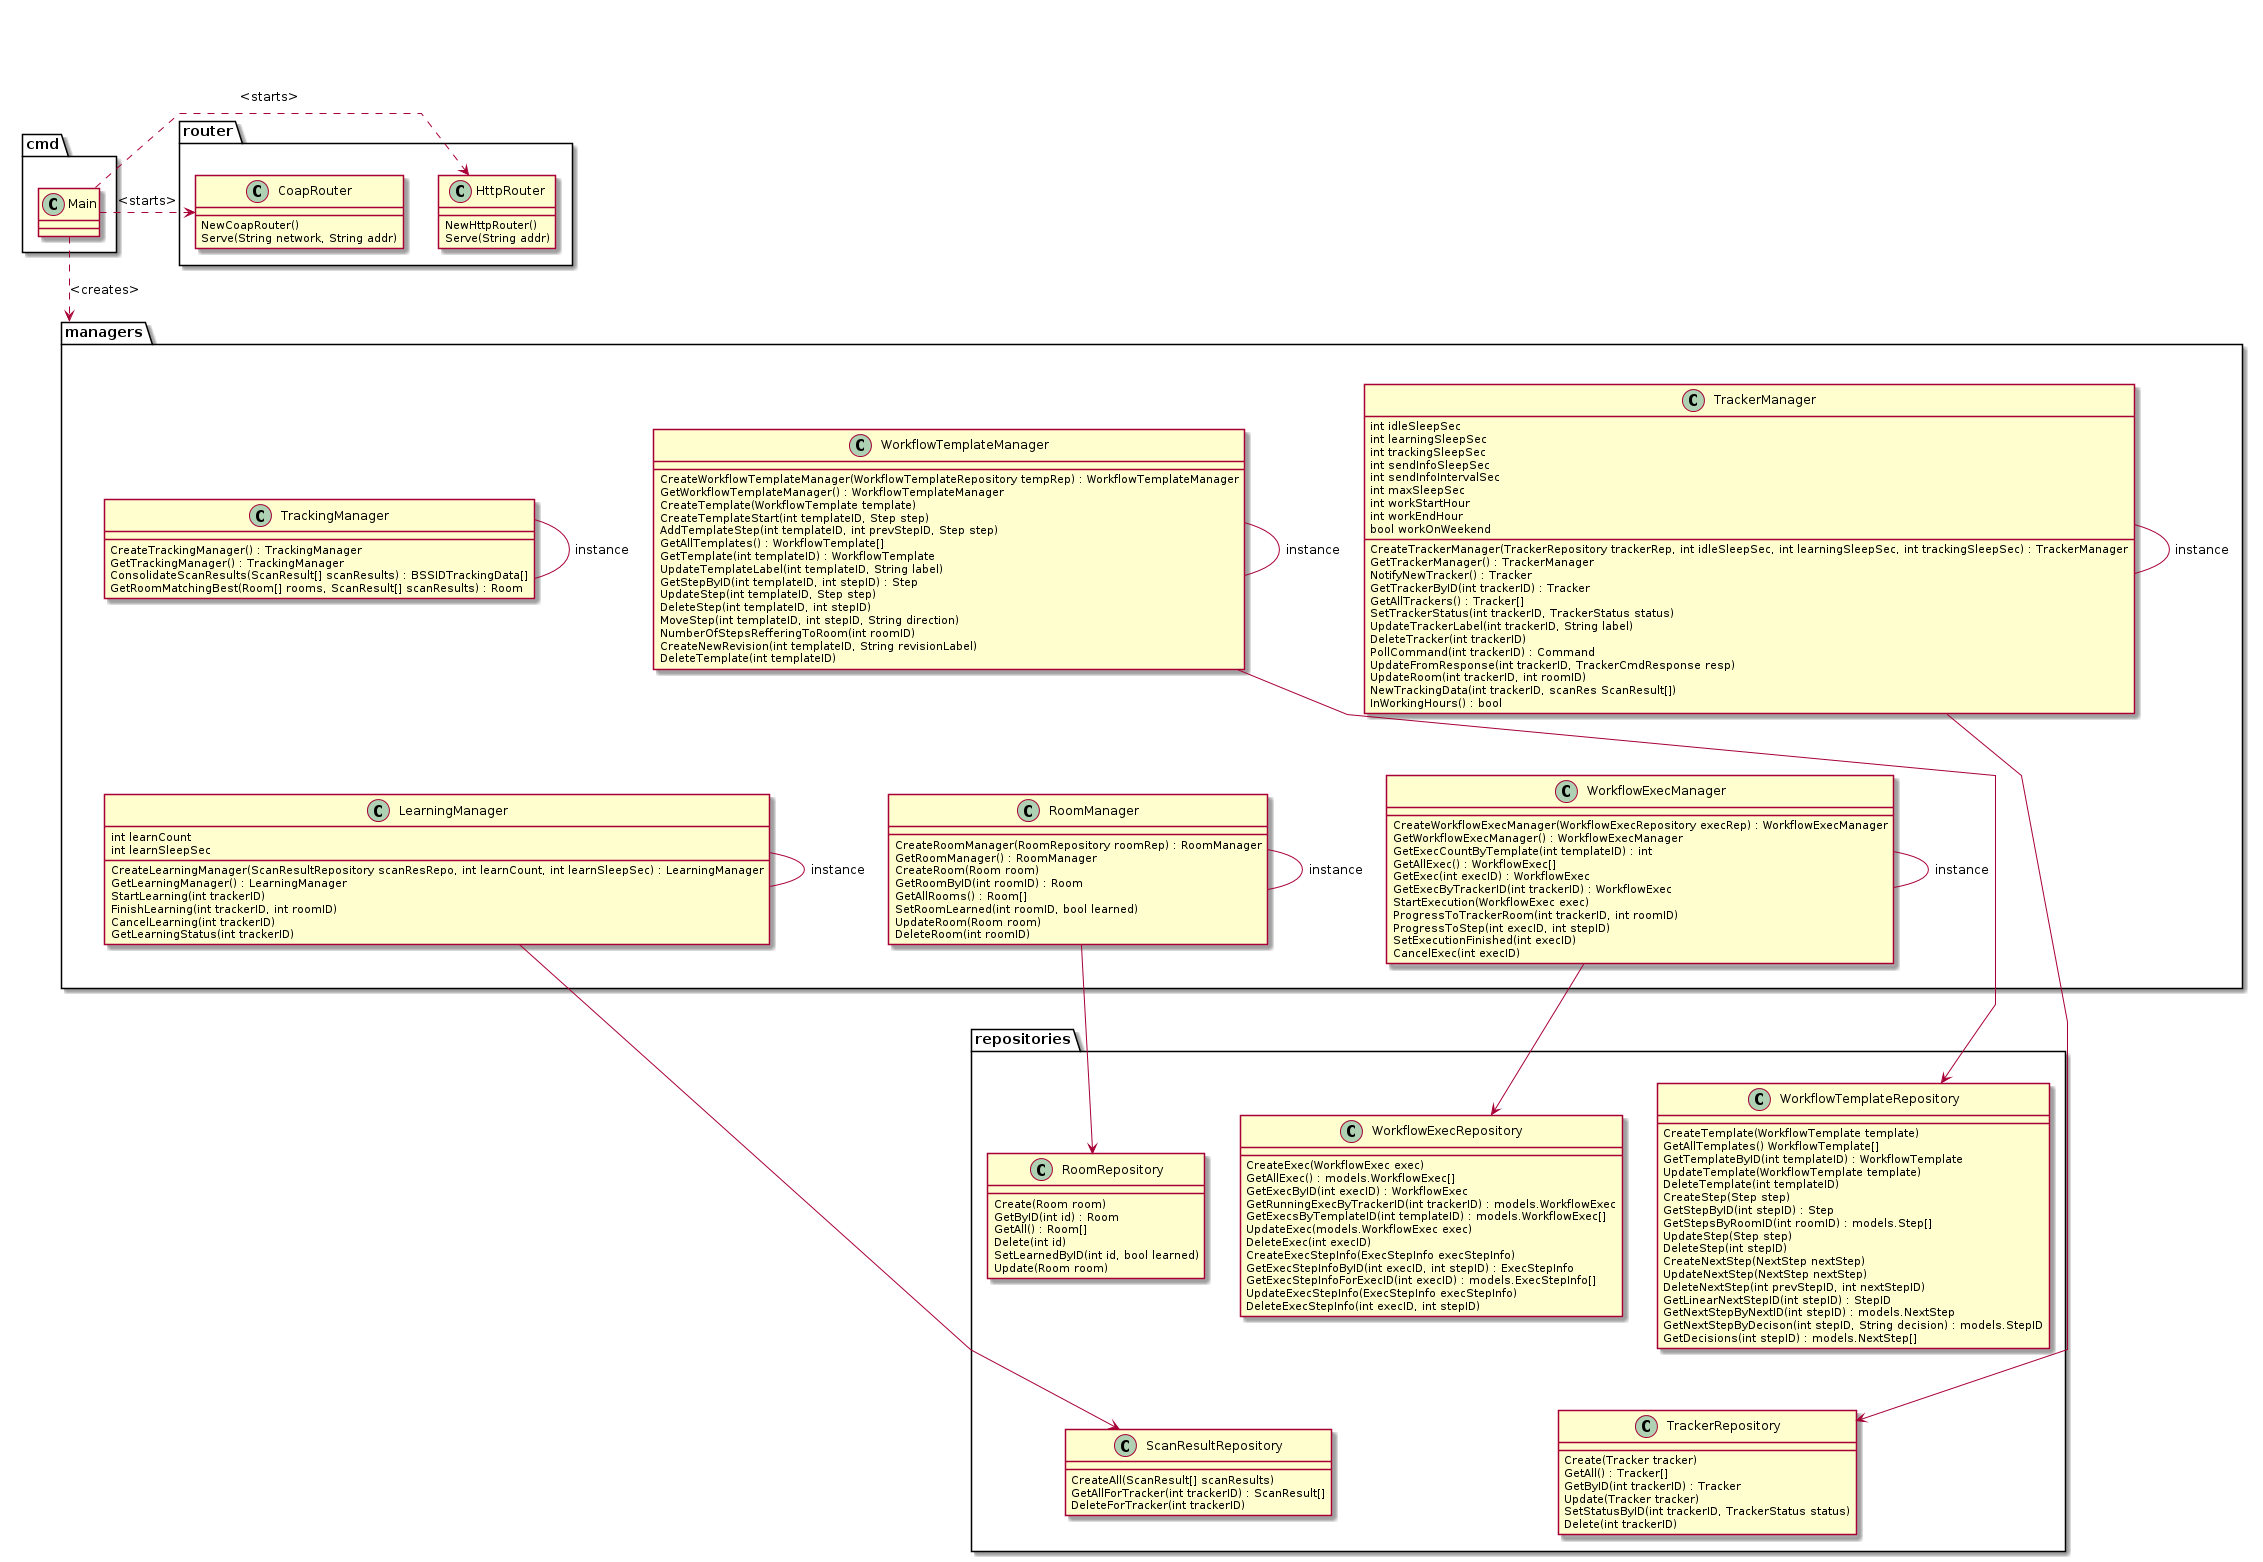
\includegraphics[width=.9\textheight]{images/server_architecture.png}
	\caption{Software-Architektur für die Backend-Anwendung}
	\label{fig:software-architecture}
\end{sidewaysfigure}

\FloatBarrier
\subsubsection{Tracker Lokalisierung}

Die raumgenaue Lokalisierung eines Trackers besteht aus zwei Teilen.
Der erste Teil ist das Einscannen eines Raumes mit Hilfe eines Trackers und der zweite das Zuordnen von Scanergebnissen
zu einem zuvor eingescannten Raum.

Beim Einscannen eines Raumes werden von einem Tracker, wie bei der eigentlichen Lokalisierung, Scanergebnisse angefordert.
Dies soll mehrfach über einen größeren Zeitraum geschehen.
Die genaue Anzahl an Wiederholungen und die Pause zwischen Scans soll konfigurierbar sein.
Nach den Scans liegen für alle verfügbaren \glspl{BSSID} ein oder mehrere \glspl{RSSI} (also Signalstärken) vor.
Weiter gehört jede \gls{BSSID} zu einer \gls{SSID}.

Diese Daten sollen im nächsten Schritt von dem Benutzer nach \glspl{SSID} gefiltert werden, die für die Lokalisierung
genutzt werden sollen.
Dadurch können zum Beispiel mobile \gls{WLAN}-Netzwerke von Smartphones, die nicht permanent vorhanden sind, herausgefiltert werden.
Dies verhindert ein Fehlschlagen einer Lokalisierung, wenn ein mobiles Netzwerk nicht verfügbar ist.

Nach der Filterung werden aus den mehreren \glspl{RSSI} pro \gls{BSSID} statistische Kenngrößen berechnet.
Diese werden im zweiten Teil für die Lokalisierung verwendet.
Berechnet werden, wie die Klasse \enquote{BSSIDTrackingData} zeigt:
\begin{itemize}
	\item Minimum
	\item Maximum
	\item Arithmetisches Mittel
	\item Median
	\item Erstes Quartil
	\item Drittes Quartil
\end{itemize}

Soll nun ein Tracker lokalisiert werden, werden von diesem wieder Scanergebnisse angefordert.
Dies liefert pro \gls{BSSID} einen \gls{RSSI}-Wert.
Um nun einen \enquote{besten} Raum aufgrund dieser Werte dem Tracker zuzuweisen, soll ein Scoring-System verwendet werden.
Dafür wird zuerst jedem Raum ein Score zugewiesen.
Die genaue Berechnung für diesen Wert soll während der Implementierung über verschiedene Tests herausgefunden werden.
Grob soll zum Beispiel für jeden \gls{RSSI}-Wert, der innerhalb des gespeicherten Minimum und Maximum dieser \gls{BSSID}
eines Raumes liegt, eine gewisse Punktzahl vergeben werden.
Auch sind Punkte je nach Abstand vom Mittelwert und/oder Median denkbar.

Erhält ein Raume eine Punktzahl über einem bestimmten Schwellwert, ist dieser ein Kandidat für den Raum, in dem der Tracker
sich befindet.
Letztendlich wird der Raum gewählt, der über dem Schwellwert liegt und insgesamt die meisten Punkte erhalten hat.
Dieser Raum kann dann als aktueller Raum des Trackers eingetragen werden und für den Fortschritt einer Workflow-Ausführung
verwendet werden.

\subsubsection{Daten-Export}

Für einen Daten-Export muss zuerst ausgewählt werden, welche Daten exportiert werden sollen.
Da der Export des Paper-Trackers bei einer Optimierung der Workflows helfen soll, müssen hauptsächlich Daten der
Klassen \enquote{WorkflowTemplate}/\enquote{WorkflowExecution} und derem Umfeld exportiert werden.
Konkret wären dies die Templates, deren Ausführungen inklsuive detailierter Infos der Schritte (\enquote{ExecStepInfo}).
Diese Informationen können helfen, langsame oder nicht benötigte Schritte eines Workflows zu identifizieren.

Weiter sollen auch Informationen zu den Revisionen eines Templates exportiert werden.
Anhand dieser Informationen kann verfolgt werden, ob Anpassungen eines Workflows einen Erfolg gebracht haben.
Dazu müssen zu den Revisionen einige Metriken erfasst werden.
Die zu erfassenden Metriken sind:
\begin{itemize}
	\item Anzahl der Ausführungen
	\item Prozentzahl der erfolgreich abgeschlossenen Ausführungen
	\item Durchschnittliche Dauer einer Ausführung
\end{itemize}

Mit der Auswahl der Daten kann auch das Format des Exports ausgewählt werden.
Alle zu exportierenden Daten können sehr gut in Tabellen exportiert werden.
Dies führt zu hauptsächlich zwei Exportformate: \gls{CSV} und Excel.

\gls{CSV} ist ein weit verbreitetes und simples Format, da es hauptsächlich mit Kommas (',') und Zeilenumbrüchen arbeitet.
Dadurch ist es sehr einfach zu erstellen und einzulesen.
Die meisten Tools, die mit solchen Daten arbeiten, haben die Möglichkeit \gls{CSV}-Dateien einzulesen.
Ein großer Nachteil von \gls{CSV} ist jedoch, dass es nicht standardisiert ist und mehrere Arten
mit kleinen Unterschieden existieren \cite{rfc4180}.
Im RFC-4180 werden lediglich scheinbar übereinstimmende Teile der verschiedenen Implementierungen dargestellt.
Nach diesen gibt es einen weiteren Nachteil: Pro \gls{CSV}-Datei kann nur eine Tabelle gespeichert werden.
Dies würde für den Export des Paper-Trackers bedeuten, dass entweder mehrere Dateien oder eine gebündelte Datei angeboten werden muss.

Excel oder genauer das von Excel verwendete \enquote{xlsx}-Format ist ein offenes und standardisiertes Format
für Kalkulationstabellen \cite{iso29500}.
Da es ein offenes Format ist, kann es auch von anderen Programmen, wie Libre Office, geöffnet und bearbeitet werden.
Es muss nicht, wie bei \gls{CSV} erst importiert werden.
Auch unterstützt es mehrere Tabellen in einer Datei, welches den Download des Exports vereinfacht.
Aus diesen Gründen wird Excel als Exportformat für den Paper-Tracker verwendet.

\FloatBarrier
\subsection{App für Mobilgeräte} \label{sec:app}

Die App für Mobilgeräte soll dem Endbenutzer die Möglichkeit geben, alles um den Paper-Tracker und die damit verbundenen Workflows einzusehen und zu bearbeiten.
Sie soll dafür die oben erwähnte \gls{REST}-Schnittstelle nutzen und deren Operationen dem Endbenutzer zur Verfügung stellen.

Die Oberfläche selbst soll möglichst intuitiv sein.
Um dies zu erreichen, wurden als Entwurf für die App einige Design-Prototypen erstellt, welche die grundlegenden Elemente der App darstellen.
Diese Prototypen wurden zum Teil per Hand auf Papier gezeichnet und zum Teil digital entworfen.

Alle Designs wurden größtenteils mit Designelementen entworfen, die im zu verwendenden \gls{UI}-Framework vorhanden sind.
Daher wurden auf Bausteine des
Flutter-Frameworks\footnote{https://flutter.dev/docs/development/ui/widgets} zurückgegriffen, welche
sich an die von Google entworfene Material-Designsprache halten. (vgl. \cite{Google2020})
Im Folgenden werden einige dieser Prototypen vorgestellt.

\FloatBarrier
\subsubsection{Hauptseite}

In \autoref{fig:ui-main-page} ist der Prototyp der Hauptseite der App zu sehen.
Die Hauptseite ist der zentrale Einstiegspunkt der App und bietet eine Übersicht über grundlegende
Informationen.

Allgemein ist die Hauptseite in einen Kopfbereich und einen Inhaltsbereich aufgeteilt.
Der Kopfbereicht zeigt lediglich den Titel der App \enquote{Paper-Tracker} an und einen Button, mit dem das Tutorial aufgerufen werden kann.
Das Tutorial ist weiter in \autoref{sec:app-tutorial} beschrieben.
Im Inhaltsbereich gibt es weiter eine Aufteilung in verschiedene Tabs, die jeweils für eine Klasse im Datenmodell stehen.
Es soll einen Tab für Workflows in der Ausführung, Workflow-Templates, Räume und Tracker geben.
Jeder Tab und damit jede Klasse soll ein eindeutiges Icon zugewiesen bekommen, mit dem die Klassen auf verschiedenen Seiten der App wiedererkannt werden können.
Die Tabs sollen über ein Wischen nach links und rechts oder über ein Auswählen in der Tableiste gewechselt werden können.

In den Tabs wird eine Liste aller Objekte der entsprechenden Klasse mit den wichtigsten dazugehörigen Informationen angezeigt.
Dies ist zum Beispiel für einen Tracker der aktuelle Raum oder der Batteriestatus.

Über ein Pull-Down\footnote{Herunterziehen der Liste über den eigentlichen Inhalt hinaus.} der jeweiligen Liste, kann diese aktualisiert werden.
Wenn der Nutzer einen Eintrag der Liste auswählt, soll sich eine Detailseite zu diesem Objekt öffnen.
Ein Design-Prototyp dazu ist in \autoref{sec:app-room} dargestellt.

Unten rechts in der Ecke ist ein \enquote{Floating Action Button} untergebracht.
Über diesen soll ein Dialog geöffnet werden, in dem ein neues Objekt der entsprechenden Klasse erzeugt werden kann.
Dazu ist weiter unten in \autoref{sec:app-dialog} auch ein Design-Prototyp beschrieben.

\begin{figure}[h!tbp]
	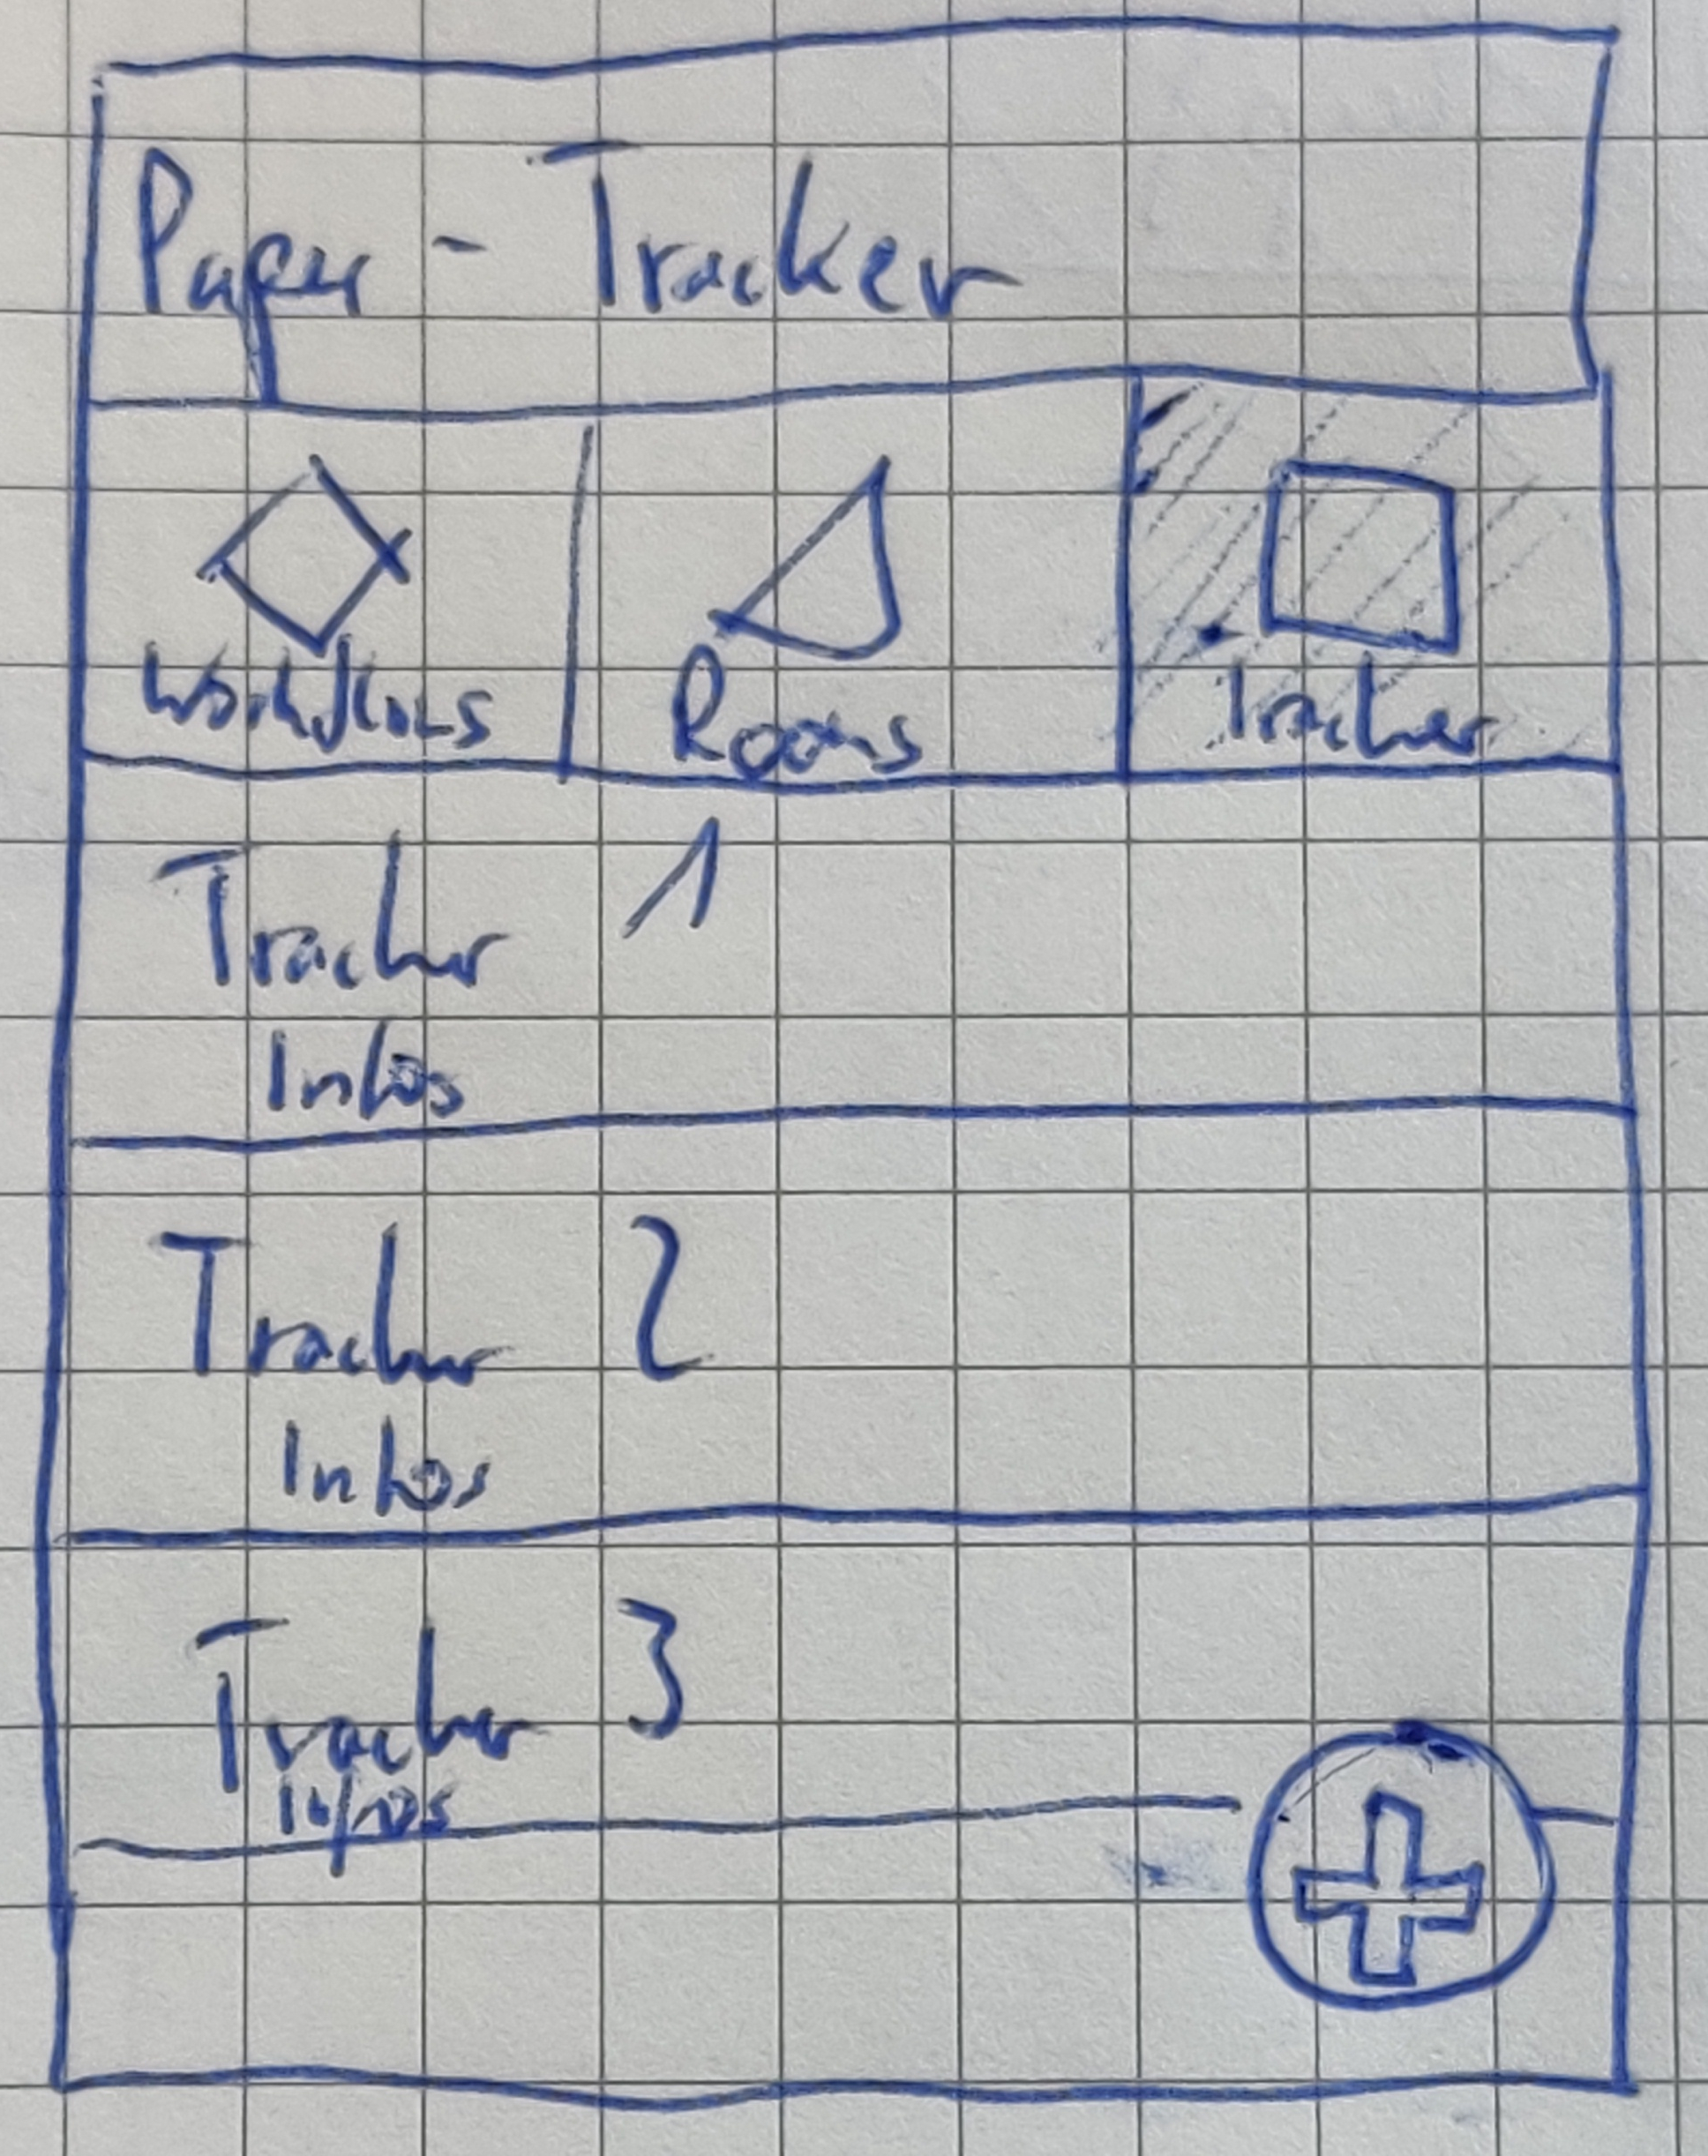
\includegraphics[width=.4\textwidth]{images/ui-prototype/main_page.jpg}
	\centering
	\caption{Design-Prototyp der Hauptseite}
	\label{fig:ui-main-page}
\end{figure}

\FloatBarrier

\subsubsection{Darstellung von Workflows}

\autoref{fig:ui-workflow} zeigt den Prototyp für die Darstellung von Workflows.
Dies können sowohl Workflows in der Ausführung als auch Templates sein.

Die einzelnen Schritte eines Workflows sollen als Boxen in einer Liste dargestellt werden.
Der Nutzer muss in dieser Liste scrollen können, falls es in einem Workflow zu viele Einzelschritte
gibt, um diese auf einem Bildschirm anzeigen zu können.
Als letzte Box in der Liste wird ein Button angezeigt, mit dem der Nutzer einen neuen Schritt an die Liste anhängen kann.
Die Eingabe der Informationen des neuen Schritts soll in einem Dialog erfolgen.
Diese Box wird nur angezeigt, falls der anzuzeigende Workflow bearbeitbar ist.
\TODO{Ist schon irgendwo erläutert, wann ein Workflow nicht mehr bearbeitbar ist?}

In den Boxen zu den Schritten sollen einige Informationen angezeit werden.
So werden beispielsweise der Name des Schrittes, der dem Schritt zugewiesenen Raum und die
verfügbaren Optionen dargestellt.
Die Optionen sind jeweils einzelne Buttons.
Durch ein Auswählen eines Options-Button, werden die zu diesem Button gehörenden Schritte unter dem Schritt eingerückt angezeigt.
Diese Schritte werden wie oben beschrieben in einer identischen Liste angezeigt und unterstützen auch das Einfügen neuer Schritte.

\begin{figure}[h!tbp]
	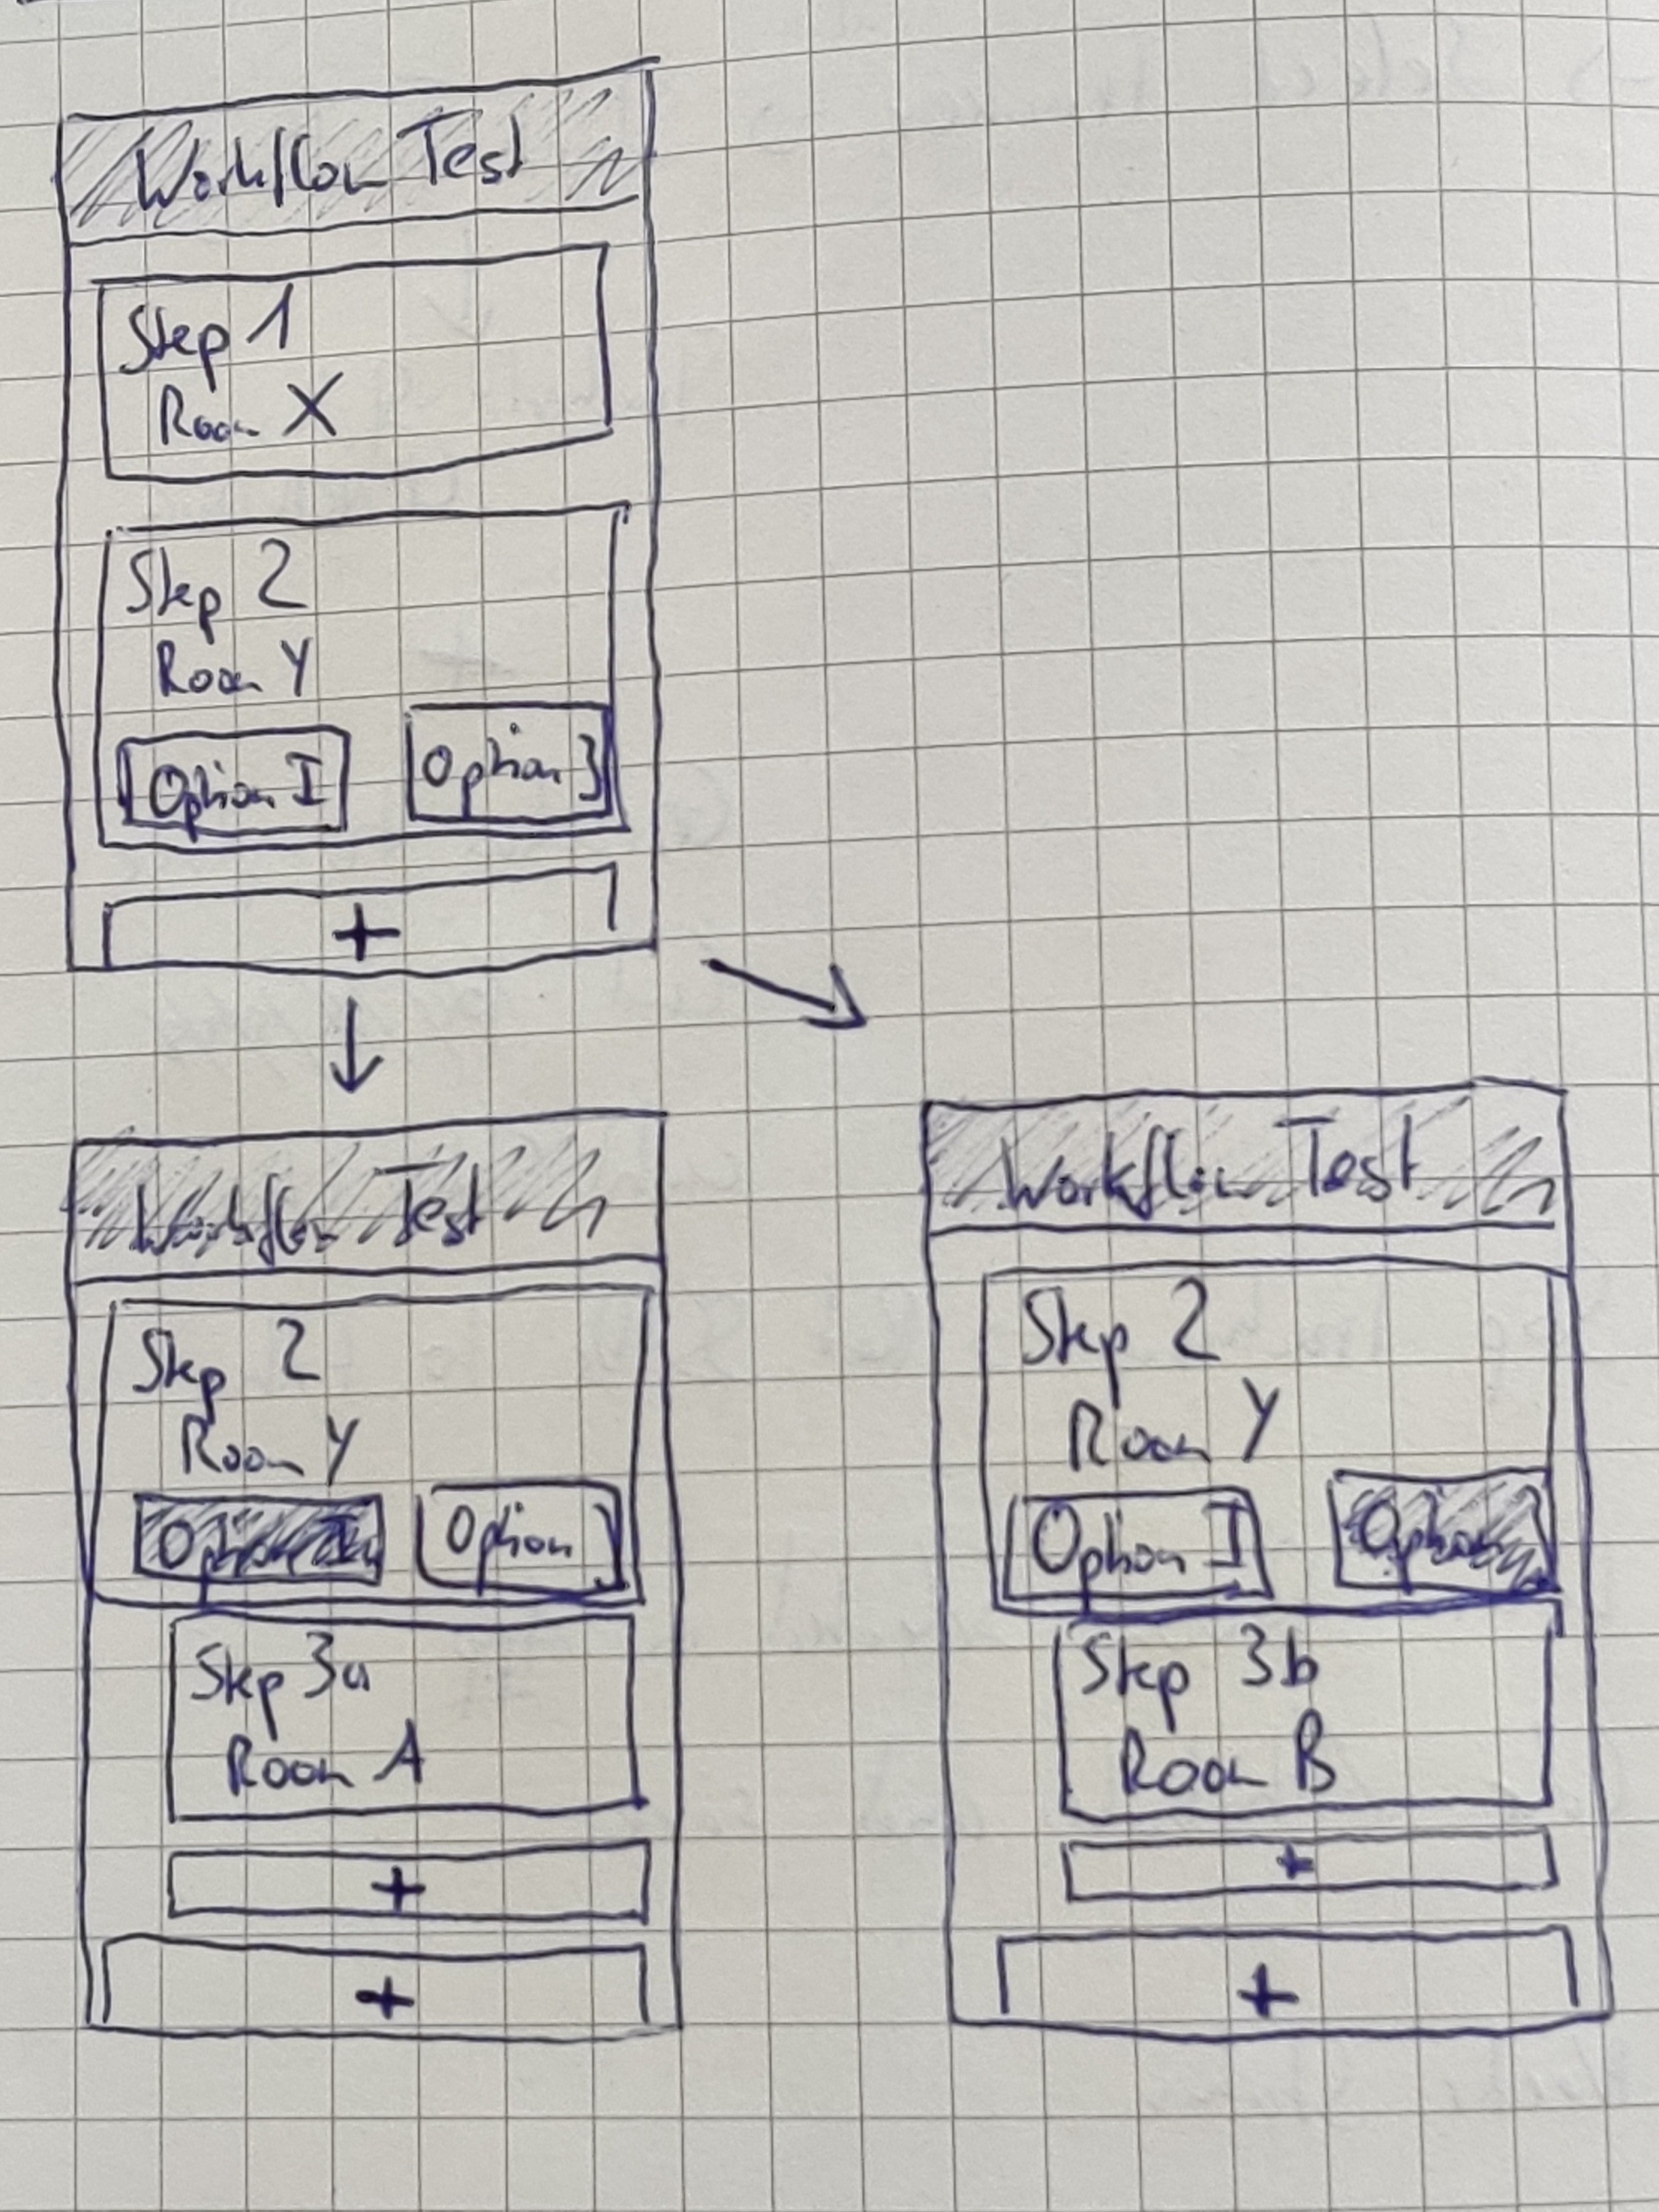
\includegraphics[width=.7\textwidth]{images/ui-prototype/workflow.jpg}
	\centering
	\caption{Design-Prototyp der Darstellung von Workflows}
	\label{fig:ui-workflow}
\end{figure}

\subsubsection{Detailseite für Räume} \label{sec:app-room}
In \autoref{fig:ui-detail-page} ist der Design-Prototyp für eine Detailseite dargestellt.
Beispielhaft wird hier die Tracker-Detailseite behandelt.

Im Kopfbereich der Seite ist neben einem Button für die Navigation das Icon für die Klasse Tracker und der Name des Trackers dargestellt.
Der Inhaltsbereich der Seite beihaltet eine Liste mit allen wichtigen Attributen des Trackers.
Jeder Eintrag besteht aus dem Namen des Attributs links und dem Attribut selbst rechts.
Wenn möglich soll das Attribut selbst in einem modifizierbaren Feld dargestellt werden, das vorerst gesperrt ist.

Der Fußbereich einer Detailseite besteht aus zwei Buttons.
Mit dem linken Button können die editierbaren Attribute freigeschaltet werden.
Dabei wird aus dem \enquote{Stift}-Icon ein \enquote{Speichern}-Icon und über den Button können die bearbeiteten Attribute gespeichert werden.
Der rechte Button dient zum Löschen des dargestellten Objekts.

Je nach Klasse des dargestellten Objekts ändert sich das Icon im Kopfbereich und die angezeigten Attribute.
In folgender \autoref{tab:detail-attributes} ist gelistet, für welche Klassen welche Attribute angezeigt werden und, ob diese editierbar sind.

\begin{table}[]
\centering
\begin{tabular}{l|l|r}
\textbf{Klasse}  & \textbf{Attribut} & \multicolumn{1}{l}{\textbf{Editierbar}} \\ \hline
Tracker          &                   &                                         \\
								 & Label             & Ja                                      \\
								 & Raum              & Nein                                    \\
								 & Batterie          & Nein                                    \\
								 & Status            & Nein                                    \\ \hline
Raum             &                   & \multicolumn{1}{l}{}                    \\
								 & Label             & Ja                                      \\
								 & Eingelernt        & Über Button                             \\ \hline
WorkflowTemplate &                   & \multicolumn{1}{l}{}                    \\
								 & Label             & Ja                                      \\
								 & Initiale Revision & Nein                                    \\
								 & Schritte          & siehe Workflow-Darstellung              \\ \hline
WorkflowExec     &                   & \multicolumn{1}{l}{}                    \\
								 & Status            & Nein                                    \\
								 & Schritte          & Nein
\end{tabular}
\caption{Dargestellte Attribute der Klassen}
\label{tab:detail-attributes}
\end{table}

\begin{figure}[h!tbp]
	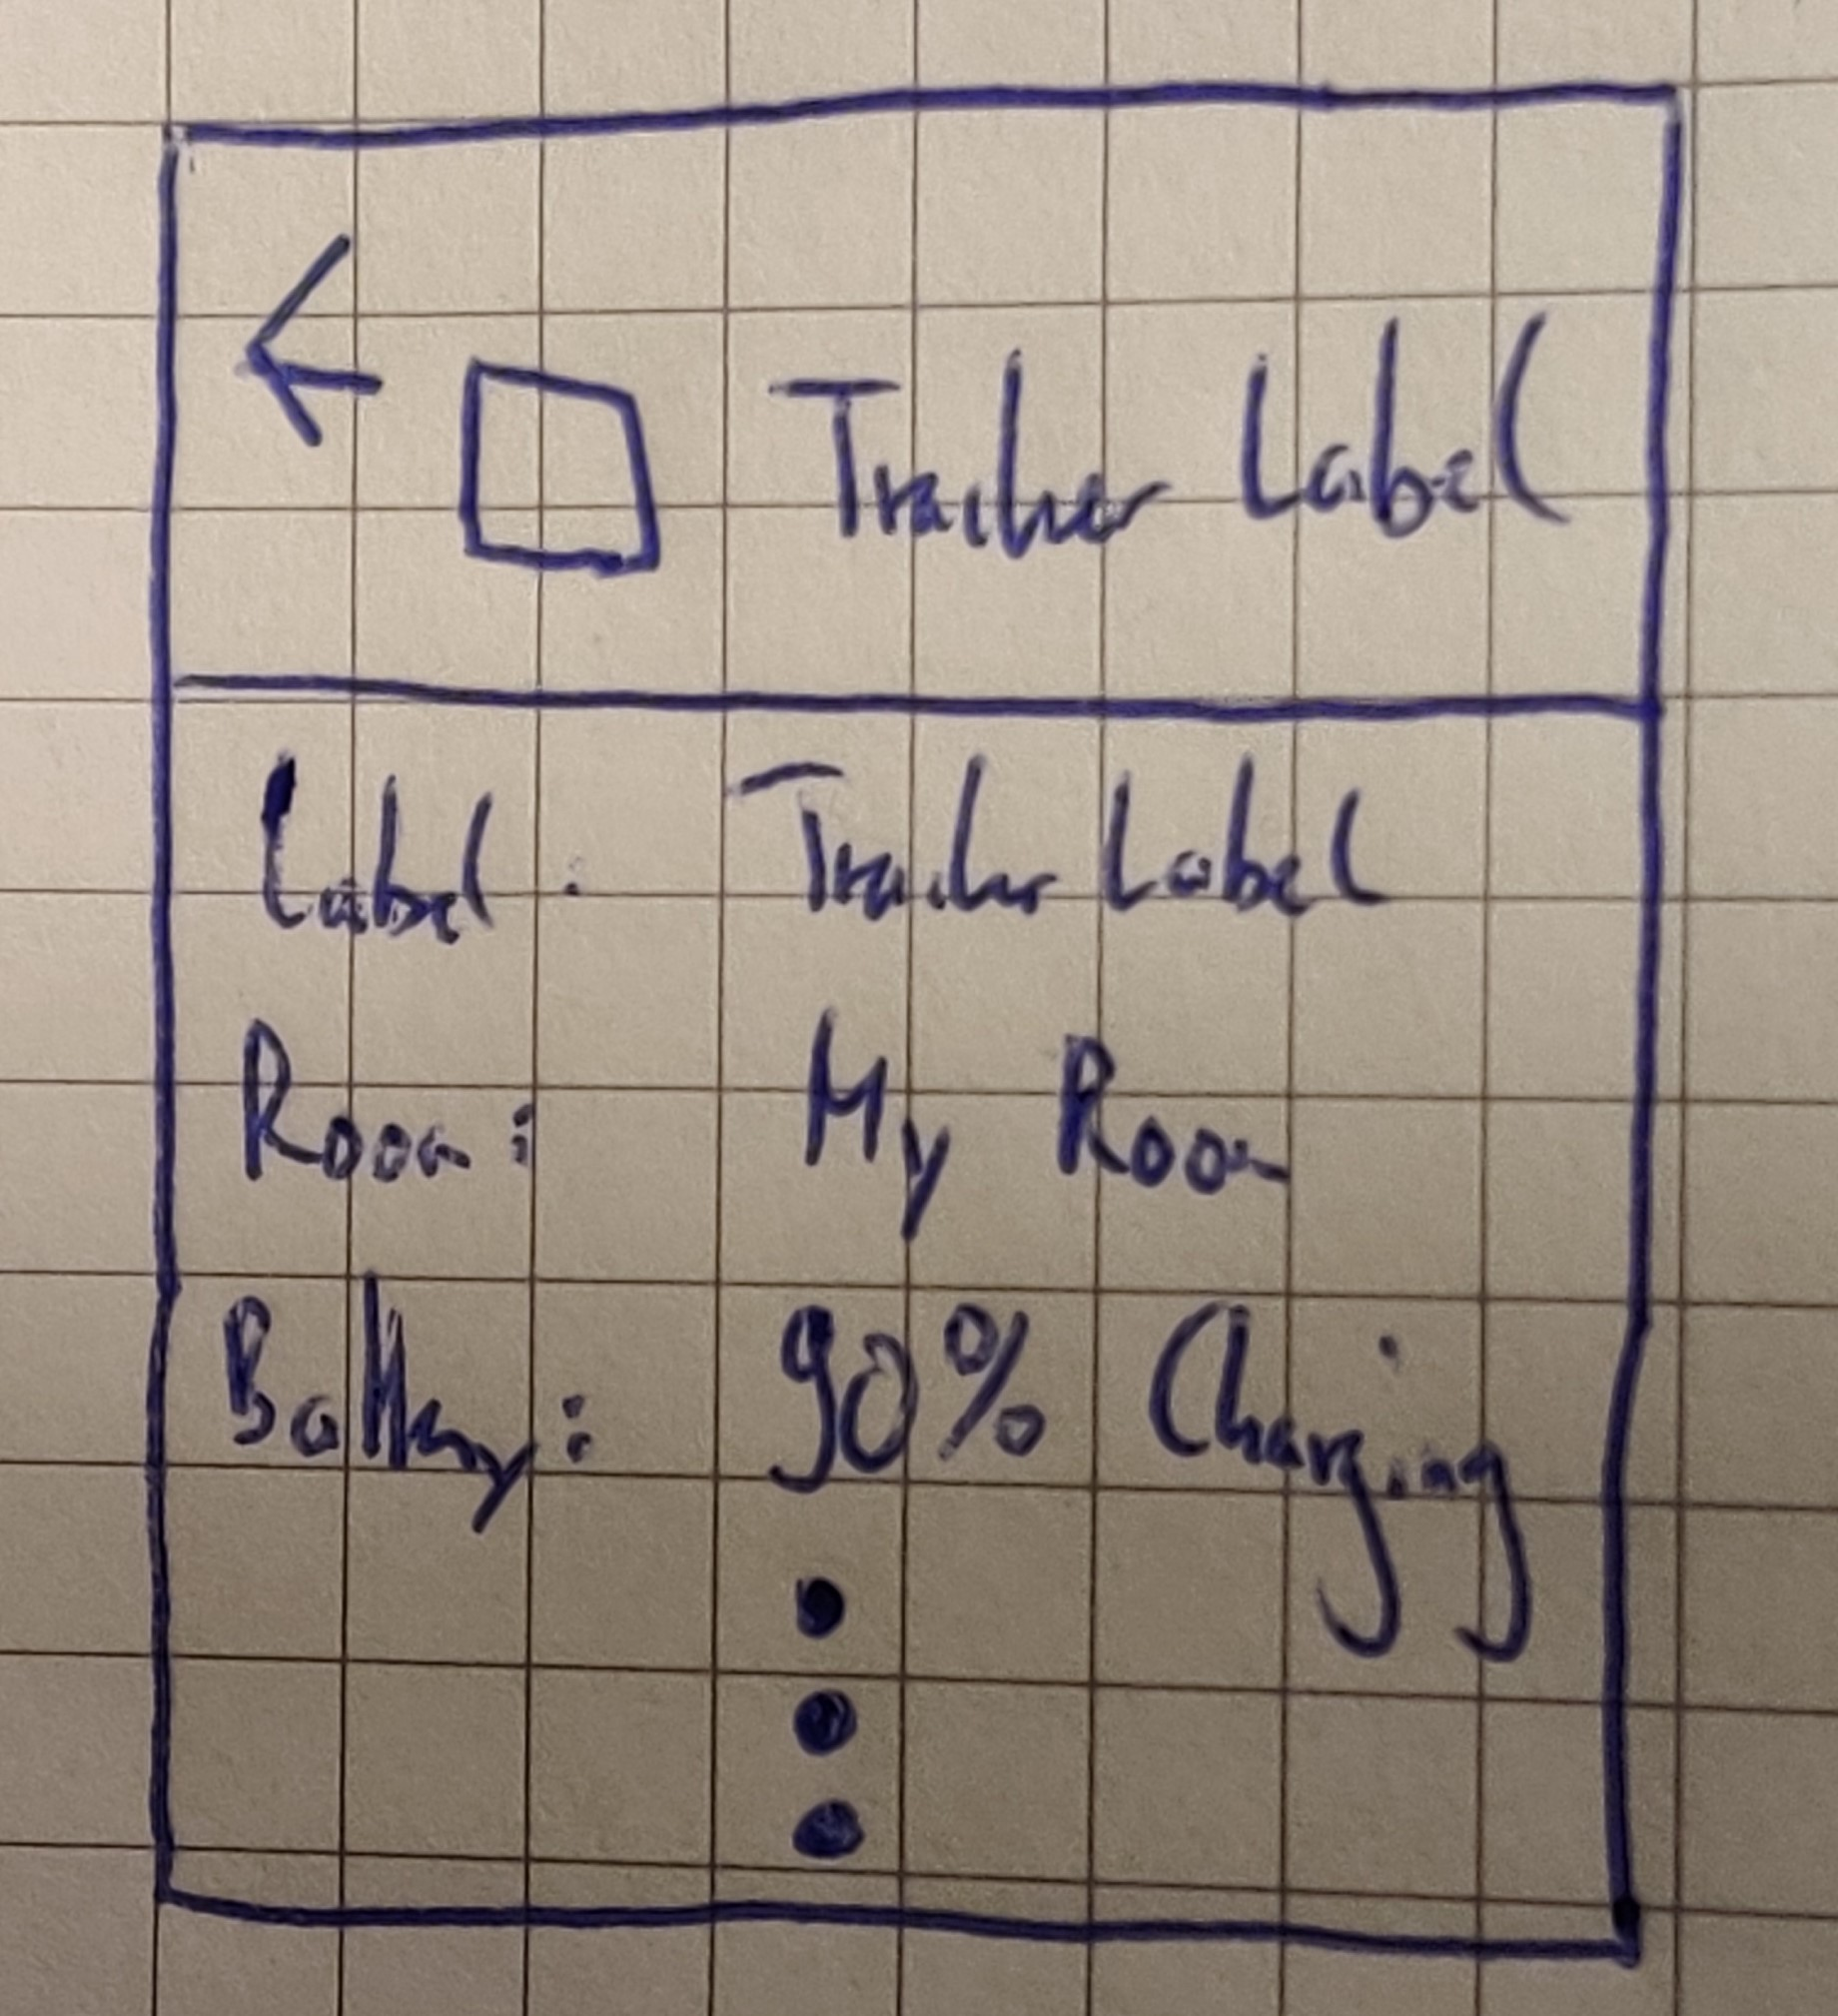
\includegraphics[width=.5\textwidth]{images/ui-prototype/detail_page.jpg}
	\centering
	\caption{Design-Prototyp der Detailseite eines Trackers}
	\label{fig:ui-detail-page}
\end{figure}

\subsubsection{Seite zum Einlernen eines Raumes}

Weiter ist in \autoref{fig:ui-learning-page} der Protoyp der Einlern-Seite dargestellt.
Auf dieser Seite kann der Endbenutzer einen Raum einlernen.
Dazu muss in zwei Dropdowns der zu lernende Raum und der zum Lernen verwendete Tracker ausgewählt werden.
Wird von einer Detailseite eines Raumes oder Trackers auf die Lernseite navigiert, so wird dieses Objekt entsprechend in einem der Dropdowns vorausgewählt.
Sind Raum und Tracker ausgewählt, kann der Einlernvorgang gestartet werden.

In diesem Fall wird statt dem Button zum Starten des Lernens eine Liste der gefundenen \glspl{SSID} angezeigt.
Der Nutzer kann in dieser Liste auswählen, welche \glspl{SSID} zum Einlernen des Raumes verwendet werden sollen.
Die Liste wird während des Vorgangs stetig mit neu gefundenen \glspl{SSID} erweitert.
Sobald der Vorgang beendet wird, kann am Ende der Seite das Einlernen über einen Button abgeschlossen werden.
Wird dieser betätigt, wird von der Seite automatisch auf die vorherige zurücknavigiert.

\begin{figure}[h!tbp]
	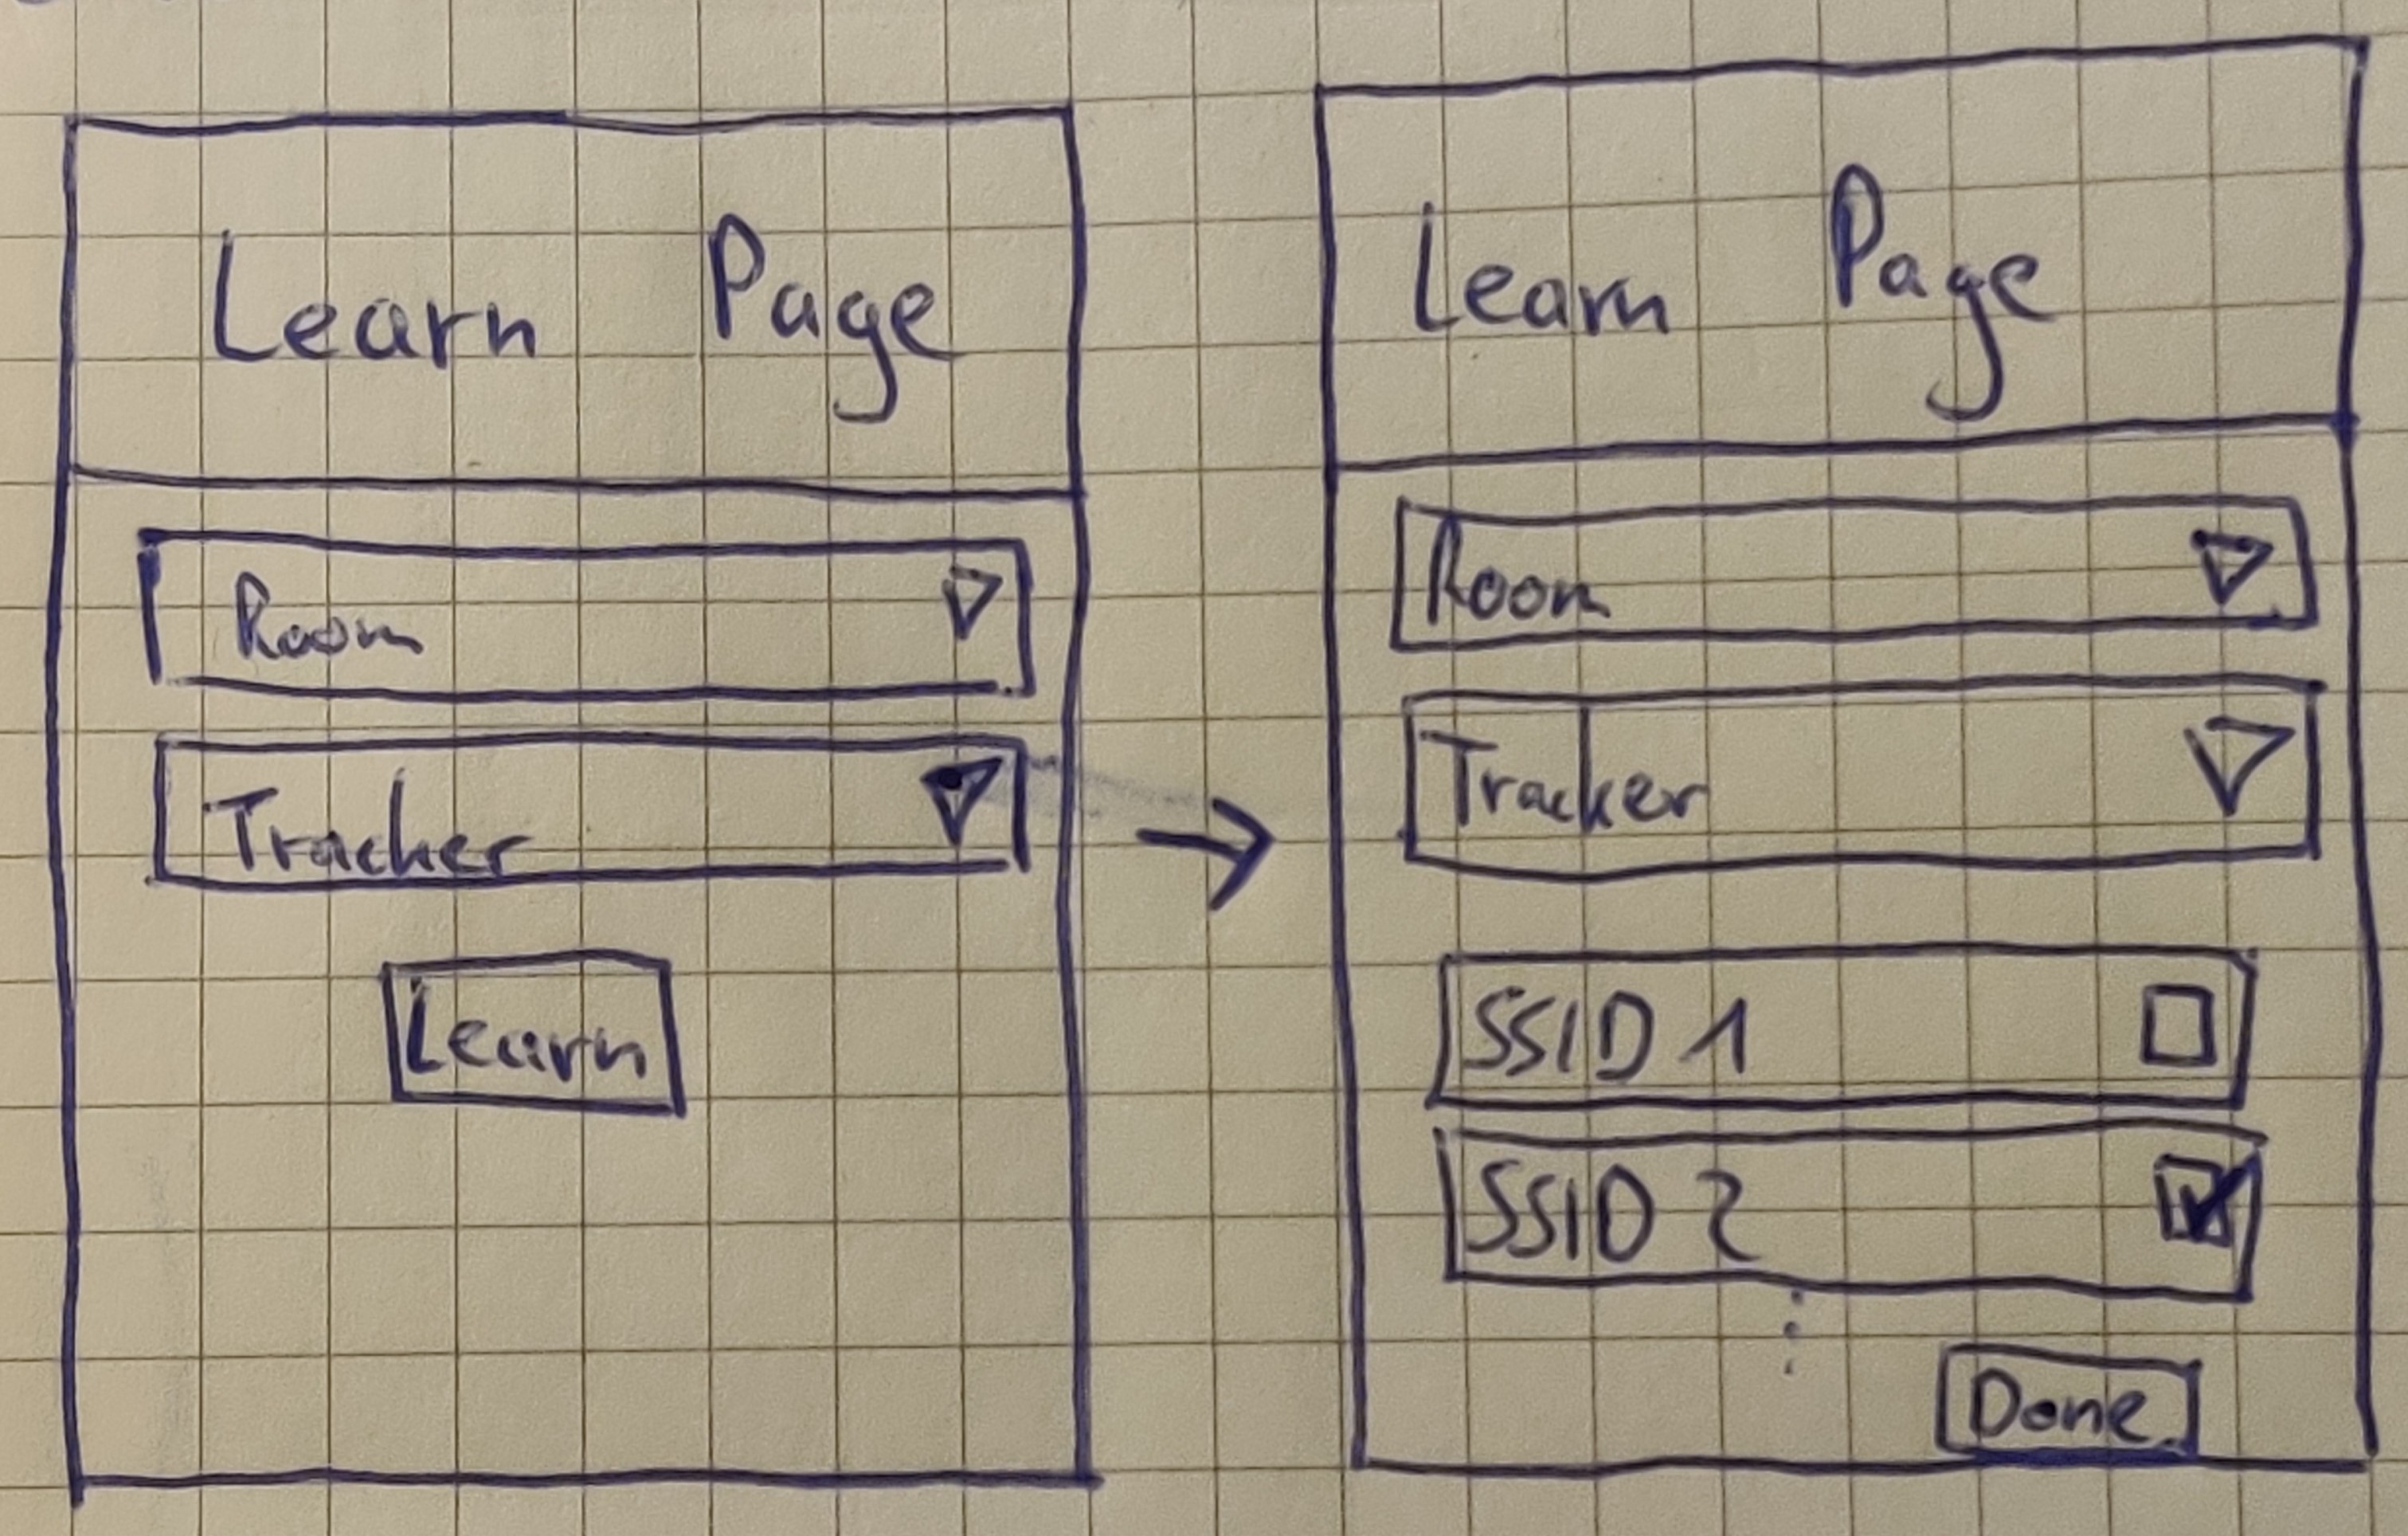
\includegraphics[width=.7\textwidth]{images/ui-prototype/learning_page.jpg}
	\centering
	\caption{Design-Prototyp der Einlern-Seite}
	\label{fig:ui-learning-page}
\end{figure}

\subsubsection{Dialoge zum Erstellen von Objekten} \label{sec:app-dialog}

Das Hinzufügen eines neuen Objektes einer Klasse kann über den \enquote{Floating Action Button} auf der Hauptseite angestoßen werden.
Durch den Button soll ein Dialog geöffnet werden, deren Design-Prototyp in \autoref{fig:ui-popup} dargestellt ist.

Der Dialog wird durch ein Pop-up realisiert.
Dieses hat eine Überschrift, die angibt welches Objekt erzeugt wird.
Unter der Überschrift können in einer Liste alle benötigten Attribute des Objekts eingegeben werden.
Wenn möglich, wie zum Beispiel bei der Auswahl eines Raumes, soll eine Dropdown-Auswahl verwendet werden.
Zu dem Dropdown soll auch wieder das Icon der Klasse, aus welcher ein Objekt ausgewählt werden soll, dargestellt werden.

\begin{figure}[h!tbp]
	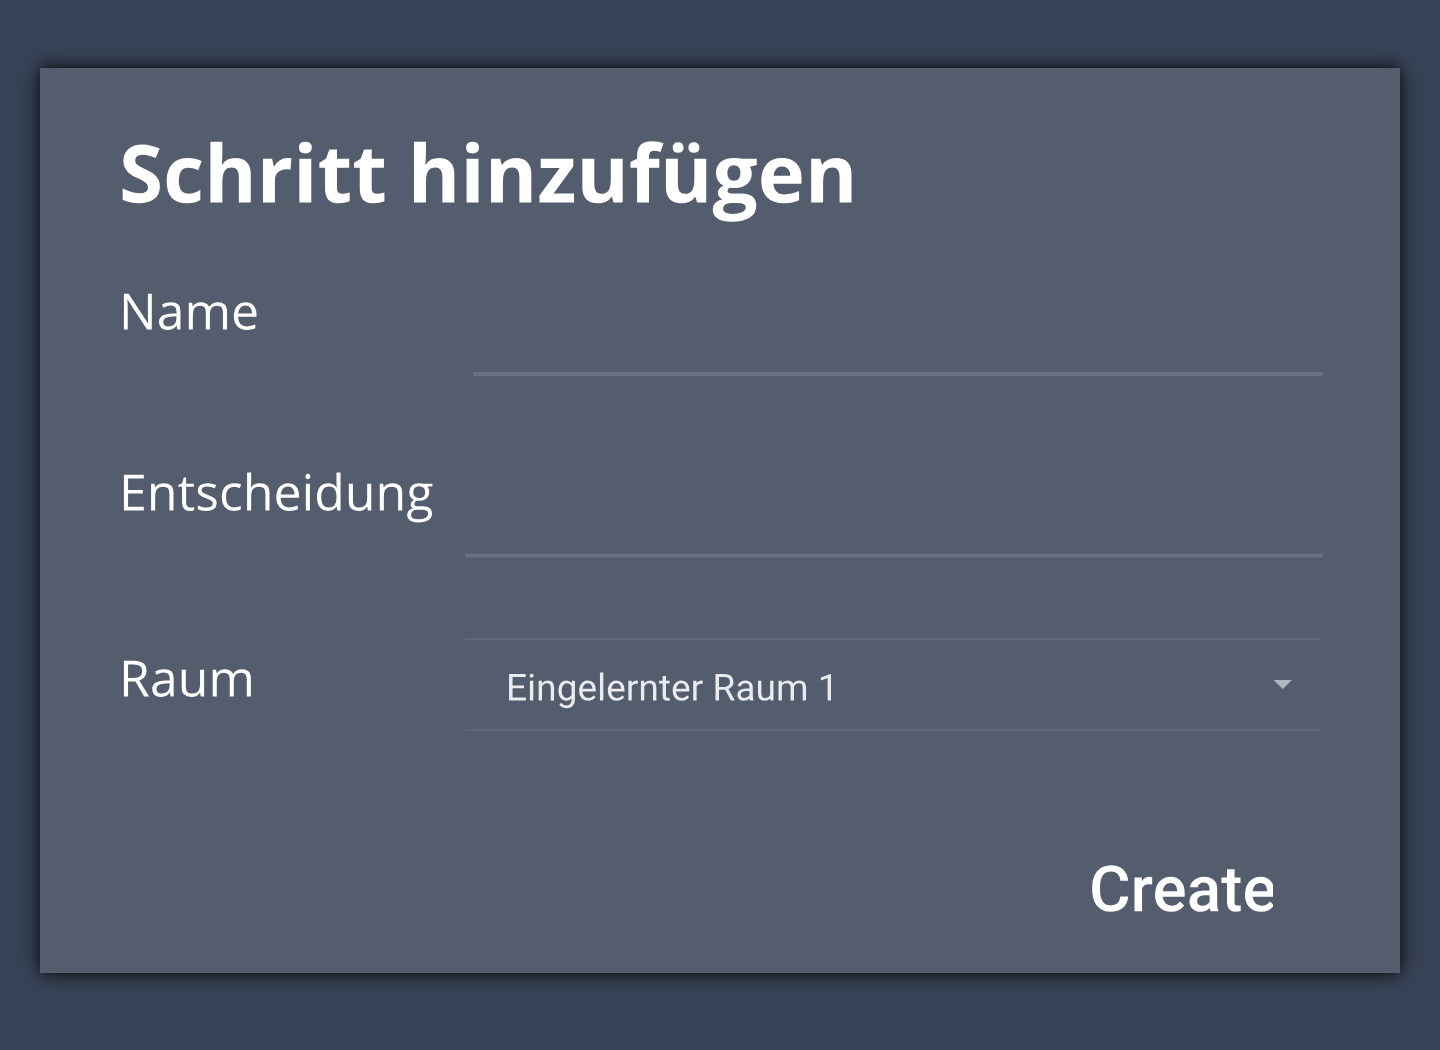
\includegraphics[width=.5\textwidth]{images/ui-prototype/popup.png}
	\centering
	\caption{Design-Prototyp eines Pop-ups zum Erstellen eines Raumes}
	\label{fig:ui-popup}
\end{figure}

\subsubsection{Tutorial-Seite} \label{sec:app-tutorial}

Beim ersten Start der App soll automatisch ein Tutorial gestartet werden, welches die Bedienung der App erklärt.
Der Nutzer soll dieses Tutorial auch von der Hauptseite aus aufrufen können.

Das Layout des Tutorials ist schlicht gehalten.
Im Zentrum ist eine Box dargestellt, in der es ein Titel, ein Bild und eine Beschreibung gibt.
Durch eine Liste an solchen Boxen kann durch ein Wischen nach links und rechts geblättert werden.
Jede Box soll mit ihrem Inhalt einen Aspekt der App näher erläutern und dem Nutzer erklären.
Unter der Box wird dem Nutzer signalisiert, wie weit dieser durch die Liste fortgeschritten ist,
indem der Index der aktuellen Box und die Gesamtzahl der Boxen angezeigt werden.
Am unteren Teil der Seite gibt es einen Button, mit dem das Tutorial beendet wird.

\begin{figure}[h!tbp]
	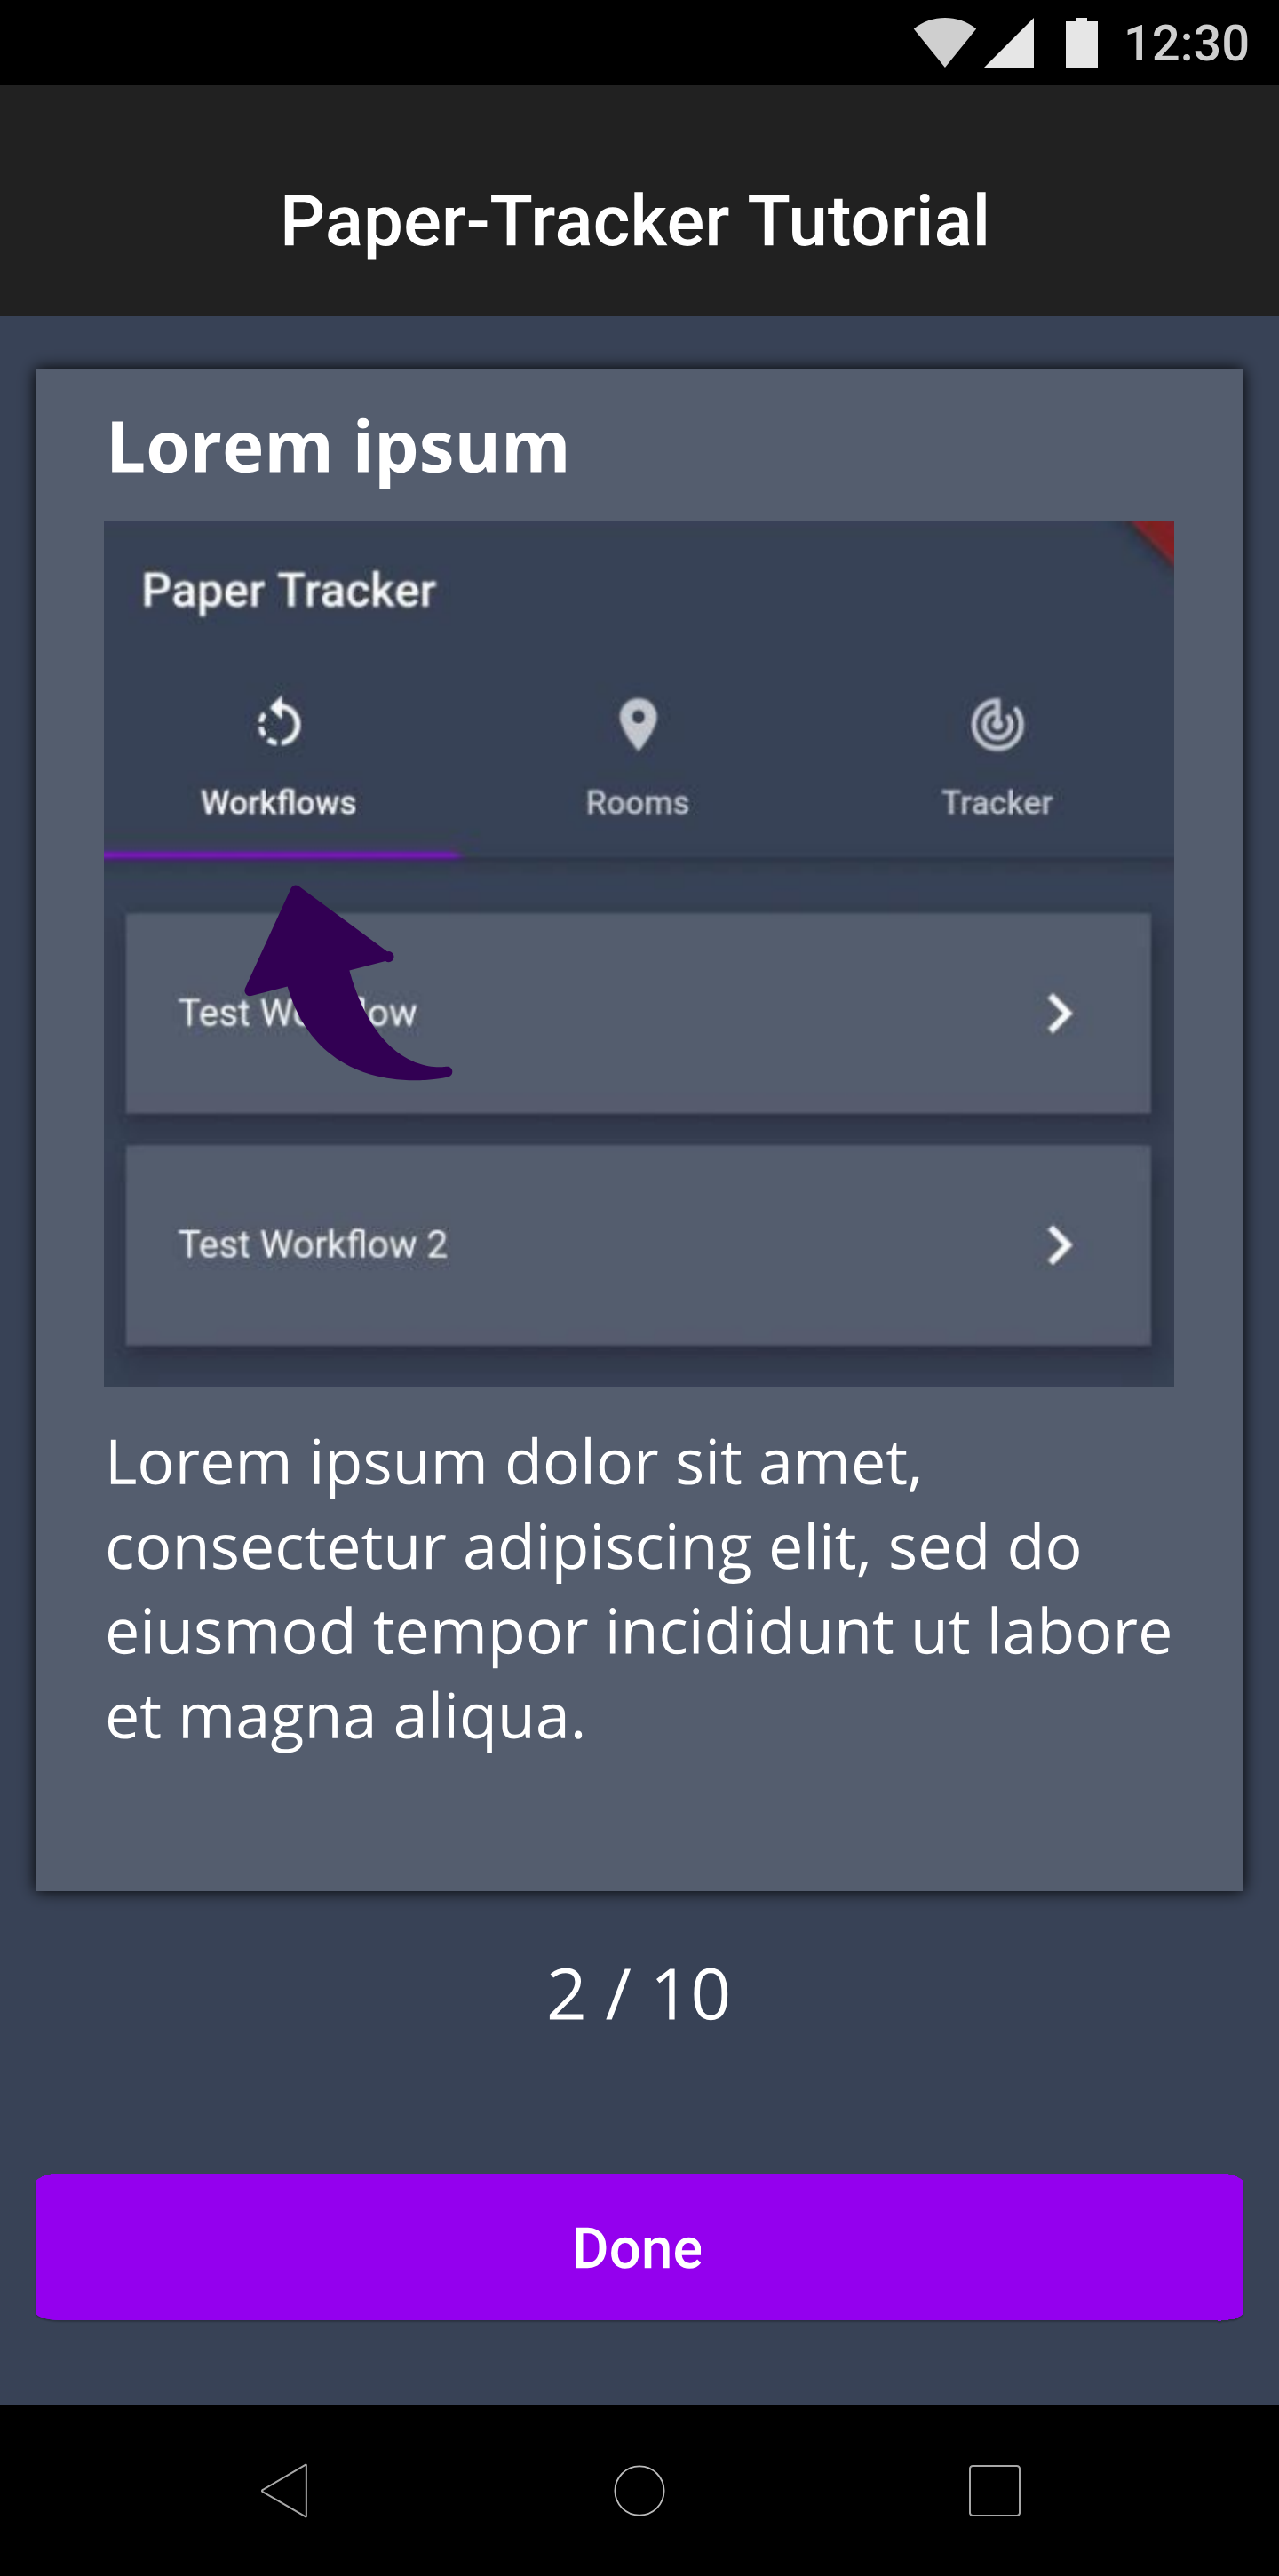
\includegraphics[height=.6\textheight]{images/ui-prototype/tutorial.png}
	\centering
	\caption{Design-Prototyp des Tutorials}
	\label{fig:ui-tutorial}
\end{figure}


\FloatBarrier

Der Inhalt des Tutorials soll alle wichtigen Funktionen der App und auch die Konfiguration des Trackers selbst abdecken.
Dafür sind die folgenden Inhalte angedacht:

\begin{enumerate}
	\item Konfiguration der App mit der Backend-Server URL mit Protokoll
	\item Hauptseite mit Unterteilung in vier Tabs und des Buttons für das Tutorial
	\item Tracker-Tab mit leerer Liste an Trackern und Hinweis, dass über den Flasher ein Tracker konfiguriert werden kann
	\item Pull-Down der Liste zum Aktualisieren. Der zuvor konfigurierte Tracker erscheint
	\item Tracker-Detailseite und das Bearbeiten eines Trackers
	\item Raum-Liste und das Erstellen eines neuen Raumes
	\item Funktionsweise des Einlernen eines Raumes
	\item Template-Liste und das Erstellen eines Templates
	\item Editieren eines Templates in der Detailseite des Templates
	\item Erstellen einer neuen Revision eines Workflow Templates
	\item Workflow-Ausführungs-Liste und das Starten einer neuen Ausführung
	\item Menü mit Aktionen zu einem Schritt in einer Workflow-Ausführung
\end{enumerate}

\subsubsection{Icons für zentrale Klassen}

\TODO{Studie über Nutzen von Icons zur Wiedererkennung von Schlüsselwörtern einbringen}

Wie schon zu der Hauptseite und Detailseite angemerkt, gibt es für jede zentrale Klasse ein zugehöriges Icon.
Die soll ermöglichen, dass der Endbenutzer in der App über die Icons die dazugehörige Klasse wiedererkennen kann.
So kann direkt erkannt werden, welcher Objekttyp auf der Detailseite angezeigt wird, oder welche
Objekte in einem Dropdown ausgewählt werden.
Zusätzlich kann das Icon abgeändert werden, wenn sich zum Beispiel der Zustand eines Objektes ändert.
Dies wird bei der Workflow-Ausführung verwendet, die ein anderes Icon besitzt, falls die Ausführung abgeschlossen ist.
Eine Übersicht der zu verwendenden Icons ist in \autoref{fig:ui-icons} gegeben.

\begin{figure}[h!tbp]
	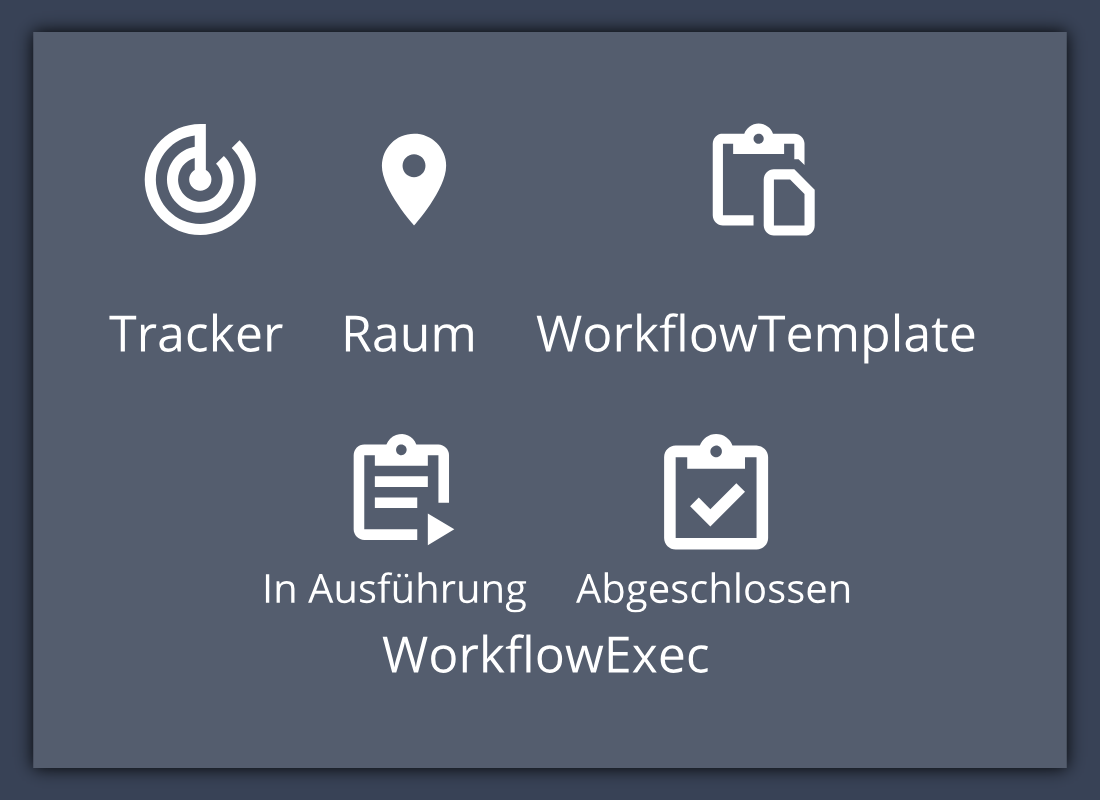
\includegraphics[height=150px]{images/ui-prototype/class-icons.png}
	\centering
	\caption{Icons für Klassen}
	\label{fig:ui-icons}
\end{figure}

\subsection{Flasher-Tool}
Da das Flasher-Tool nicht zu den Hauptkomponenten des Paper-Trackers zählt, gibt es keinen konkreten Entwurf zum \gls{UI}-Design.
Trotzdem muss konkret definiert werden, welche Funktionalitäten das Tool beinhaltet.

Das Tool muss plattformübergreifen mit möglichst wenigen externen Abhängigkeiten gestartet werden können.
Mit dem Start der Anwendung soll der Nutzer in einem \gls{GUI} die Konfigurationsdaten für die Firmware eingeben können.
Die benötigten Konfigurationswerte sind in der folgenden Liste dargestellt:

\begin{description}
	\item[\gls{WLAN} \gls{SSID}] \hfill \\
		Name des \gls{WLAN} Netzwerkes, mit dem sich der Tracker verbinden soll
	\item[\gls{WLAN} Nutzername] \hfill \\
		Nutzername, mit dem sich der Tracker am \gls{WLAN} anmelden soll. Diese Konfiguration kann freigelassen werden, falls nur ein Passwort für die Anmeldung ausreicht.
	\item[\gls{WLAN} Passwort] \hfill \\
		Passwort, mit dem sich der Tracker am \gls{WLAN} anmelden soll.
	\item[Backend-Server \gls{IP}] \hfill \\
		Die IP-Adresse, unter welcher der Backend-Server aus dem angegebenen \gls{WLAN}-Netz erreichbar ist.
\end{description}

Neben den Konfigurationsdaten müssen noch der Ort der Firmware auf dem ausführenden Computer und der Port, an welchem die Hardware verbunden ist, angegeben werden.

Nachdem alle Konfigurationsdaten angegeben sind, soll das Tool die Hardware mit den Werten programmieren.
Dabei soll dem Nutzer der aktuelle Prozess in Form eines Fortschrittsbalken oder durch Anzeige von Protokollen visualisiert werden.
